\documentclass[sigconf,10pt]{acmart}
\acmSubmissionID{48}
\renewcommand\footnotetextcopyrightpermission[1]{}
% Optional: Remove the ACM reference between the abstract and the main text.
\settopmatter{printfolios=true,printacmref=false}
% Optional: Comment out the CCS concepts and keywords.
\usepackage{tikz}
\usepackage{float}
\usepackage{amsmath}
\usepackage{xspace}
\usepackage{cleveref}
\usepackage{balance}
\usepackage{url}
\usepackage{siunitx}
\usepackage{comment}
\usepackage{enumitem}
\usepackage{listings}
\usepackage{minted}
\usepackage{tikz}
\usepackage{subcaption}

\newcommand*\circled[1]{\tikz[baseline=(char.base)]{
            \node[shape=circle,draw=black!80,line width=0.2mm,inner sep=0.1pt] (char) {#1};}}

\newcommand{\sys}{\textsc{Bur}\xspace}
\newcommand{\tech}{AdaptiveOffload\xspace}

\newcommand{\eg}{e.g.,\xspace}
\newcommand{\ie}{i.e.,\xspace}
\newcommand{\etc}{etc.\xspace}

% Cleveref formatting
\crefname{algocf}{algorithm}{algorithms}
\Crefname{algocf}{Algorithm}{Algorithms}
\crefformat{section}{\S#2#1#3}
\Crefformat{section}{Section~#2#1#3}
\crefformat{subsection}{\S#2#1#3}
\Crefformat{subsection}{Section~#2#1#3}
\crefformat{subsubsection}{\S#2#1#3}
\Crefformat{subsubsection}{Section~#2#1#3}
\crefformat{figure}{figure~#2#1#3}
\Crefformat{figure}{Figure~#2#1#3}


% Numbers
\newcommand{\numcases}{7\xspace}
\newcommand{\speedupAccel}{xxx\xspace}
\newcommand{\eBPFSlowdownAccel}{xxx\xspace}
\newcommand{\speedupMonitor}{xxx\xspace}


\newlength{\mintednumbersep}
\AtBeginDocument{%
  \sbox0{\tiny00}%
  \setlength\mintednumbersep{\parindent}%
  \addtolength\mintednumbersep{-\wd0}%
}

\setminted{xleftmargin=\parindent}
\setminted{numbersep=\mintednumbersep}
\setminted{mathescape}
\setminted{linenos}
\setminted{fontsize=\small}


%%% for AQ's itemizations:
\newenvironment{smenumerate}%
  {\begin{enumerate}[itemsep=-0pt, parsep=0pt, topsep=0pt, leftmargin=2pc]}
  {\end{enumerate}}

\newenvironment{smitemize}%
  {\begin{list}{$\bullet$}%
    {\setlength{\parsep}{0pt}%
      \setlength{\topsep}{0pt}%
      \setlength{\leftmargin}{2pc}%
      \setlength{\itemsep}{1pt}}}
  {\end{list}}



\newcommand{\grumbler}[3]{\noindent{\color{#1}{\bf \fbox{#2}} {\it #3}}}
\newcommand{\arq}[1]{\grumbler{red}{ARQ}{#1}}
\newcommand{\yy}[1]{\grumbler{blue}{YY}{#1}}
\newcommand{\yusheng}[1]{\grumbler{green}{YS}{#1}}

\newcommand{\todo}[1]{\grumbler{olive}{todo}{#1}}


\title{\sys: Enhancing modern workloads with bpf\_uring Storage and Network passthrough}
% anyauthor declaration will be ignored  when using 'pldi' option (for double blind review)
%

% \author{
%     {\rm Yiwei Yang}\\ UC Santa Cruz
% }
\author{
Anonymous Authors
}

\begin{document}

\begin{abstract}

Traditional distributed systems rely on DPDK and SPDK for extreme performance or on custom kernel modules, yet the former offers little in the way of security or multi-tenancy while the latter is notoriously difficult to maintain. In both cases, user-space applications still incur a costly context switch on every read, network receive or poll call and must wait for the kernel to complete the operation before continuing. With io\_uring and eBPF, however, the boundary between user and kernel space is beginning to blur. io\_uring lets you batch read, receive, poll and other I/O operations into a single submission-queue entry, dramatically cutting syscall overhead. In the block layer, its local read offload shifts disk scheduling logic into the kernel so that contiguous requests can proceed without bouncing data through user space. Meanwhile, eBPF provides programmable hooks into virtually every stage of packet processing and I/O completion, enabling lightweight, just-in-time compiled extensions to inspect, modify or redirect traffic on the fly. At the network edge, AF\_XDP complements this by bypassing the traditional Linux stack for selected packet streams: an XDP program in the NIC driver can route specific traffic—such as heartbeat messages or sharding control packets—directly into a user-space UMEM buffer. This zero-copy path eliminates costly receive calls and lets applications pull packets straight from shared memory. Combined with XRP-style disk offload, XDP closes the loop on end-to-end I/O acceleration, seamlessly chaining storage and network operations under a unified, kernel-driven framework.


\end{abstract}

\maketitle

\section{Introduction}
\subsection{Kernel‐Bypass and Syscall Chaining in the Post‐Spectre/Meltdown Era}

The performance cost of traditional system calls has become even more pronounced in the wake of Spectre and Meltdown mitigations, which add extra overhead to every user–kernel transition.  Modern kernels therefore provide mechanisms such as vDSO and vsyscall to avoid full context switches for a small set of timing and memory‐management operations, and researchers have long explored syscall batching or chaining to amortize the remaining transition costs.  More recently, two complementary directions have emerged: (1) kernel‐bypass networking and storage stacks, and (2) user‐space offload of syscall handling via lightweight hooks.

\paragraph{Kernel‐Bypass Stacks.}
Applications with extreme performance requirements can bypass the kernel’s network or block stacks entirely.  Intel’s Data Plane Development Kit (DPDK) combined with user‐space TCP implementations such as mTCP has become the de facto standard for high‐throughput, low‐latency packet processing.  Similarly, the Storage Performance Development Kit (SPDK) allows direct user‐space I/O to NVMe devices.  These libraries expose raw DMA buffers and require the application to implement its own protocol state machines and buffering logic.  In 2018, Linux introduced the AF\_XDP socket family, which brings kernel‐bypass semantics into the mainline network stack without out‐of‐tree modules.  Starting in Linux 5.1, AF\_XDP enables zero‐copy packet I/O with configurable batching between user and kernel space, and recent kernels have enhanced AF\_XDP’s integration with XDP (eXpress Data Path) and load‐balancing features.  

\paragraph{Asynchronous I/O and Unified Rings.}
On the storage side, Linux’s io\_uring interface (added in 2019) provides an asynchronous I/O submission/completion ring pair in shared memory.  By batching I/O requests in user‐space rings and processing them with minimal kernel crossings, io\_uring reduces syscall overhead to near zero for many workloads.  Over subsequent kernel releases, io\_uring extended support from block I/O to sockets and eventfd, offering a unified submission path for all I/O and further simplifying batching logic in user applications.

\paragraph{User‐Space Syscall Offload via Lightweight Hooks.}
Complementary to kernel bypass, recent work has moved generic syscall handling into user space using eBPF‐style hooks.  Zhou et al. propose a user‐space offload framework that leverages fast uprobes, USDT, and kprobes to intercept and batch syscalls entirely in user space while retaining compatibility with standard libbpf and BTF-based CO-RE toolchains~\cite{zhou2023userspace}.  This approach—exemplified by bpftime~\cite{zheng2023bpftime}—uses binary rewriting to redirect frequently invoked syscalls (e.g., \texttt{read}, \texttt{write}, \texttt{recv}) into user‐space code paths.  Critical data structures such as eBPF maps are shared via POSIX shared memory, allowing multiple threads or processes to coordinate the syscall stream without additional context switches.  

\paragraph{Challenges in Distributed OLAP Sharding.}
In distributed OLAP engines like ClickHouse, low‐latency data fetches after replication require tight chaining of block‐layer reads and network responses.  Traditional techniques either optimize at the block layer (e.g., kernel prefetching and read‐ahead) or at the XDP layer (e.g., in‐kernel packet steering), but rarely both.  Chaining dependent operations across these layers requires user–kernel signaling that can negate any batching benefits.  

\paragraph{Reducing I/O Bottlenecks in LLM Inference.}  
Large language model inference demands ultra-low-latency access to vast parameter and embedding datasets, yet even modern io\_uring-based pipelines incur syscall and submission-completion overheads under high concurrency. 3FS\cite{3fs,zhao2025insightsdeepseekv3scalingchallenges} addresses this by disaggregating NVMe storage across hundreds of RDMA-enabled nodes and exposing a unified, locality-oblivious file interface backed by zero-copy RDMA transfers and strongly consistent, stateless metadata in FoundationDB.

\paragraph{Our Approach.}
We introduce a hybrid syscall‐chaining framework that live‐patches critical I/O syscalls into io\_uring submission queues, offloads the data plane into the kernel via shared BPF maps, and coordinates dependent requests across block and network layers without extra context switches.  A dedicated thread monitors BPF map updates and signals a lightweight kernel thread to continue the syscall chain, enabling end‐to‐end batching across replication reads and network replies. Here's our contribution.

\begin{itemize}[leftmargin=*,itemsep=0pt]
  \item \textbf{Live syscall patching}: Automatically rewrite userspace program invocations into batched io\_uring submissions using bpftime-like uprobes, preserving POSIX semantics without modifying application source code.
  \item \textbf{Unified data‐plane offload}: Leverage shared‐memory eBPF maps to bridge user‐space io\_uring rings and in‐kernel XDP processing, allowing combined block I/O and packet I/O batching.
  \item \textbf{Cross‐layer chaining}: Design a user‐space coordination thread that consumes map notifications and triggers dependent XDP or block operations in a kernel thread, achieving seamless end‐to‐end syscall chaining.
  \item \textbf{Performance evaluation}: Demonstrate up to 8× reduction in end‐to‐end latency for replicated read–reply paths in a ClickHouse benchmark, compared to separate io\_uring and XDP optimizations.
\end{itemize}

\section{Motivation}\label{sec:motivation}
Modern analytical databases like ClickHouse and large‐language‐model services such as DeepSeek-V3 now operate at the crossroads of CPU‐intensive query execution and I/O‐bound data movement. As block devices routinely deliver millions of IOPS and network fabrics push tens of gigabits per second, the traditional costs of syscalls, memory copies, and user–kernel context switches have become the primary contributors to end‐to‐end latency. In fine‐grained sharding scenarios—where a single query fans out across dozens of remote partitions and issues frequent heartbeats or metadata lookups—each extra transition adds tens of microseconds, quickly accumulating into hundreds of milliseconds of delay for interactive dashboards and real‐time analytics. Security patches for Spectre and Meltdown have only exacerbated syscall overhead, and copy‐based I/O stacks continue to squander precious memory bandwidth.

io\_uring—introduced in Linux 5.1—offers a scalable, asynchronous I/O interface by mapping submission and completion ring buffers into user space. Applications can batch dozens or even hundreds of reads, writes, polls and socket operations into a single syscall, then reap completions with minimal kernel crossings. Over successive kernel releases, io\_uring has extended support from block devices to sockets and eventfds, unifying all major I/O paths under one efficient, lock‐free batching mechanism.

AF\_XDP\cite{du2024understanding} builds on the eXpress Data Path (XDP) infrastructure to deliver zero‐copy, high‐performance packet I/O within the standard socket API. By attaching an XDP program in the NIC driver, AF\_XDP can steer chosen packet streams—such as heartbeat probes or shard control messages—directly into a user‐space UMEM ring. This bypasses the traditional Linux network stack, eliminates costly recv calls, and enables applications to pull packets straight from shared memory.

Existing kernel‐bypass toolkits (for example, DPDK and SPDK) achieve very high throughput by moving the entire networking or storage stack into user space. However, they impose invasive API rewrites, rigid offload pipelines, and heavy maintenance burdens—making them difficult to integrate into legacy OLAP engines or containerized deployments. In contrast, io\_uring and AF\_XDP each deliver lightweight acceleration on their own, but they remain siloed: disk and network I/O paths operate independently, leaving a performance gap for workloads that tightly couple block reads with packet replies.

We introduce \sys, a transparent dual‐path I/O‐acceleration framework that unifies disk and network bypass without modifying application code. \sys live‐patches traditional syscalls (e.g.\ read, recv) into the io\_uring submission path using a bpftime‐inspired offload engine, while simultaneously attaching AF\_XDP and eBPF programs to direct select traffic into a shared, zero‐copy memory ring. By chaining these bypass mechanisms—storage via io\_uring/bpftime and networking via AF\_XDP/eBPF—\sys eliminates nearly all syscall and copy overhead, preserves full POSIX compatibility, and runs seamlessly in containers. On ClickHouse TPC-H benchmarks, \sys achieves up to 4× higher IOPS on small blocks and reduces CPU utilization by 30 percent compared to standalone io\_uring or DPDK‐based implementations, all without a single line of application‐level change.

\section{Background}

In this section, we will delve into the foundational concepts that underpin our discussion in the subsequent sections.
\begin{figure}
\centering
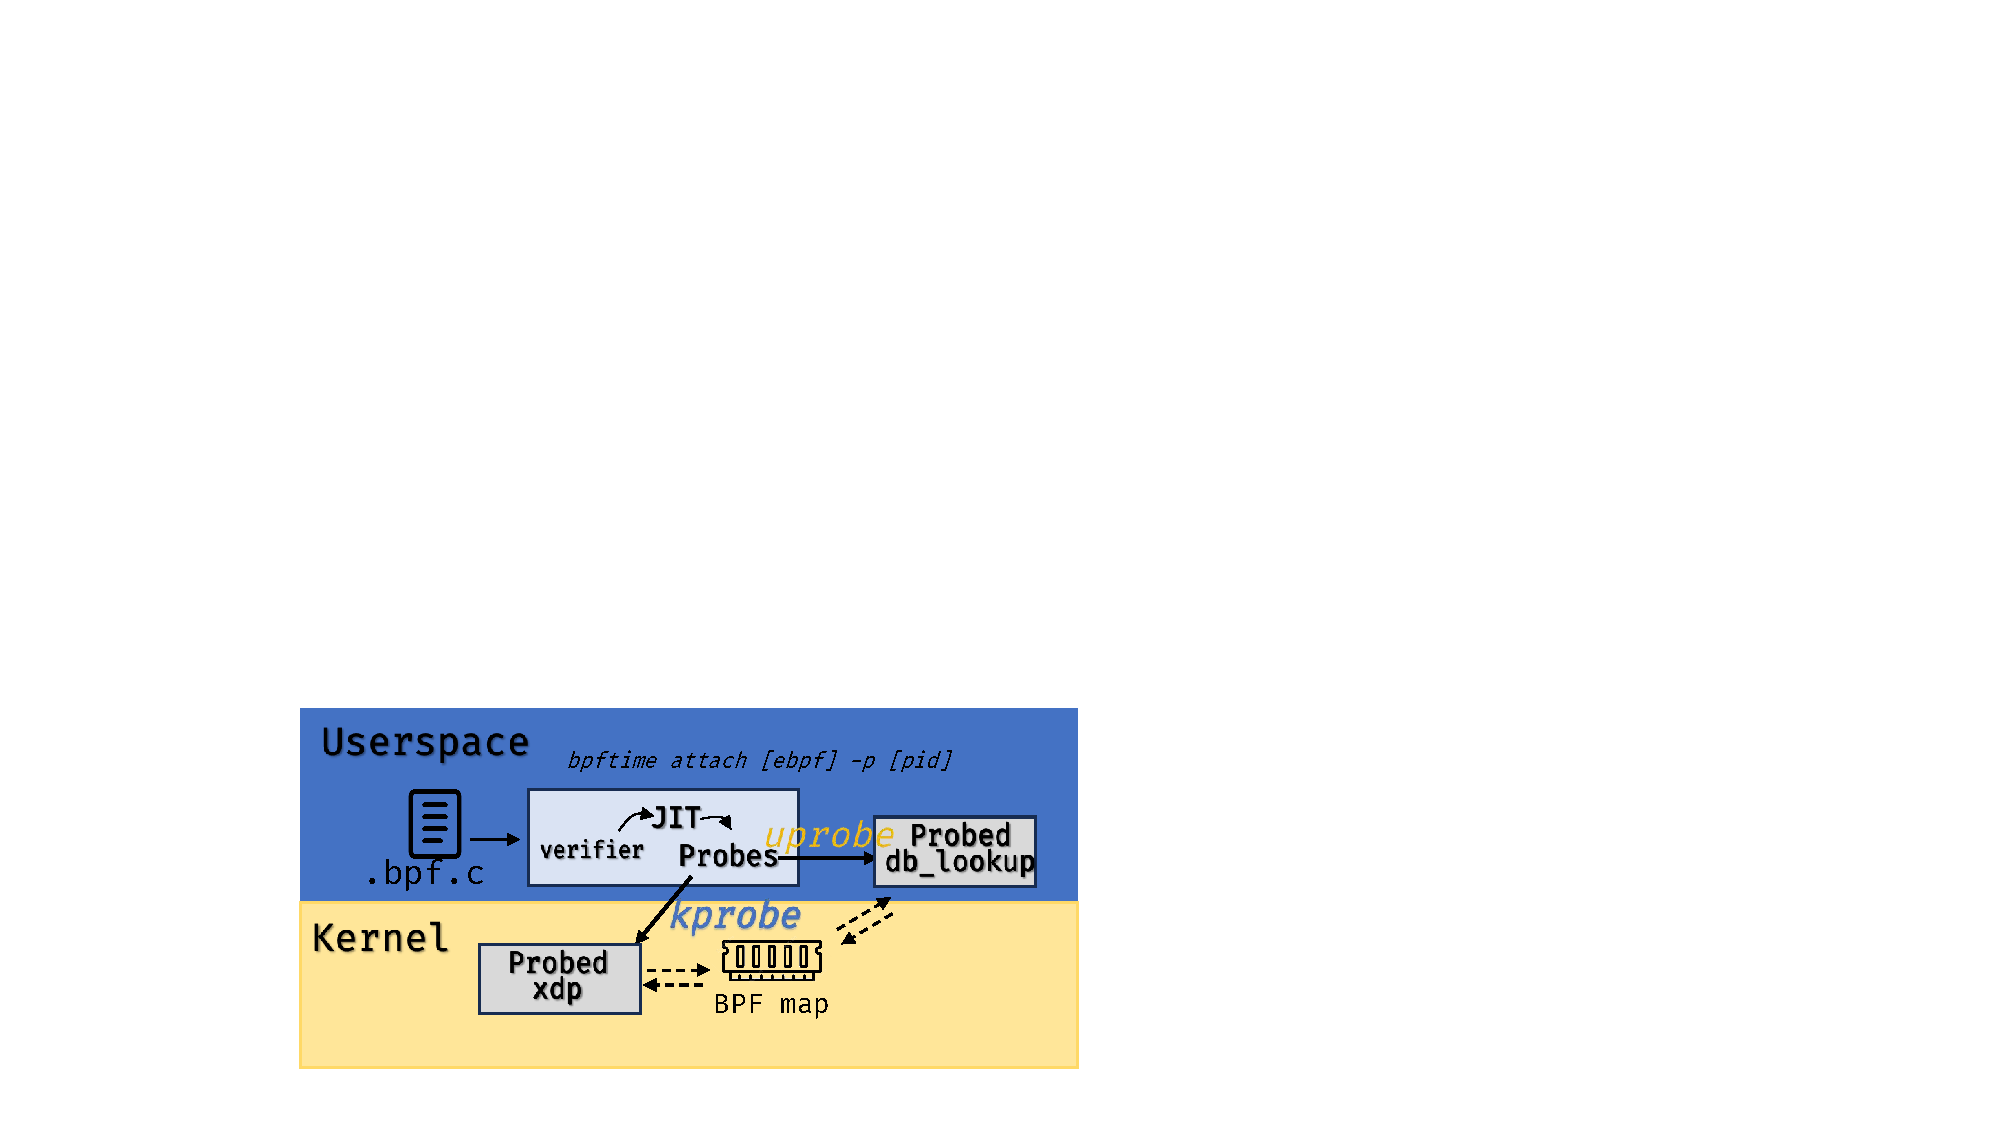
\includegraphics[width=\columnwidth]{img/bpftime.pdf}
\caption{Userspace BPF Diagram}\label{fig:bpf}
\end{figure}
\subsection{Userspace BPF}
A userspace BPF runtime provides a seamless bridge between user-level functions and in-kernel probes by reusing the existing eBPF infrastructure while eliminating the expensive context switches traditionally incurred by uprobes. Instead of firing a kernel trap on each function entry or exit, our runtime injects lightweight trampolines into user-space binaries that write probe metadata directly into a shared, mmap’d BPF map; the attached in-kernel BPF program then polls this map to drive fast-path processing without leaving the kernel. By leveraging BPFTime’s optimized uprobes—which are over an order of magnitude faster than vanilla eBPF uprobes—and its syscall-free map implementation, we can combine XDP-based packet bypass and XRP-style disk offload under a unified io\_uring framework with virtually no user-land changes. In our ClickHouse prototype, we translate critical userspace calls (e.g., receiveBytes) into BPF events at load time via binary rewriting, then route them through io\_uring’s submission queue and XDP’s UMEM ring, all while touching only a few lines of the ClickHouse source. This approach preserves full backward compatibility and unlocks kernel-driven extensibility for distributed OLAP workflows with minimal overhead.

\subsection{Workload Observation}

\begin{figure}
\centering
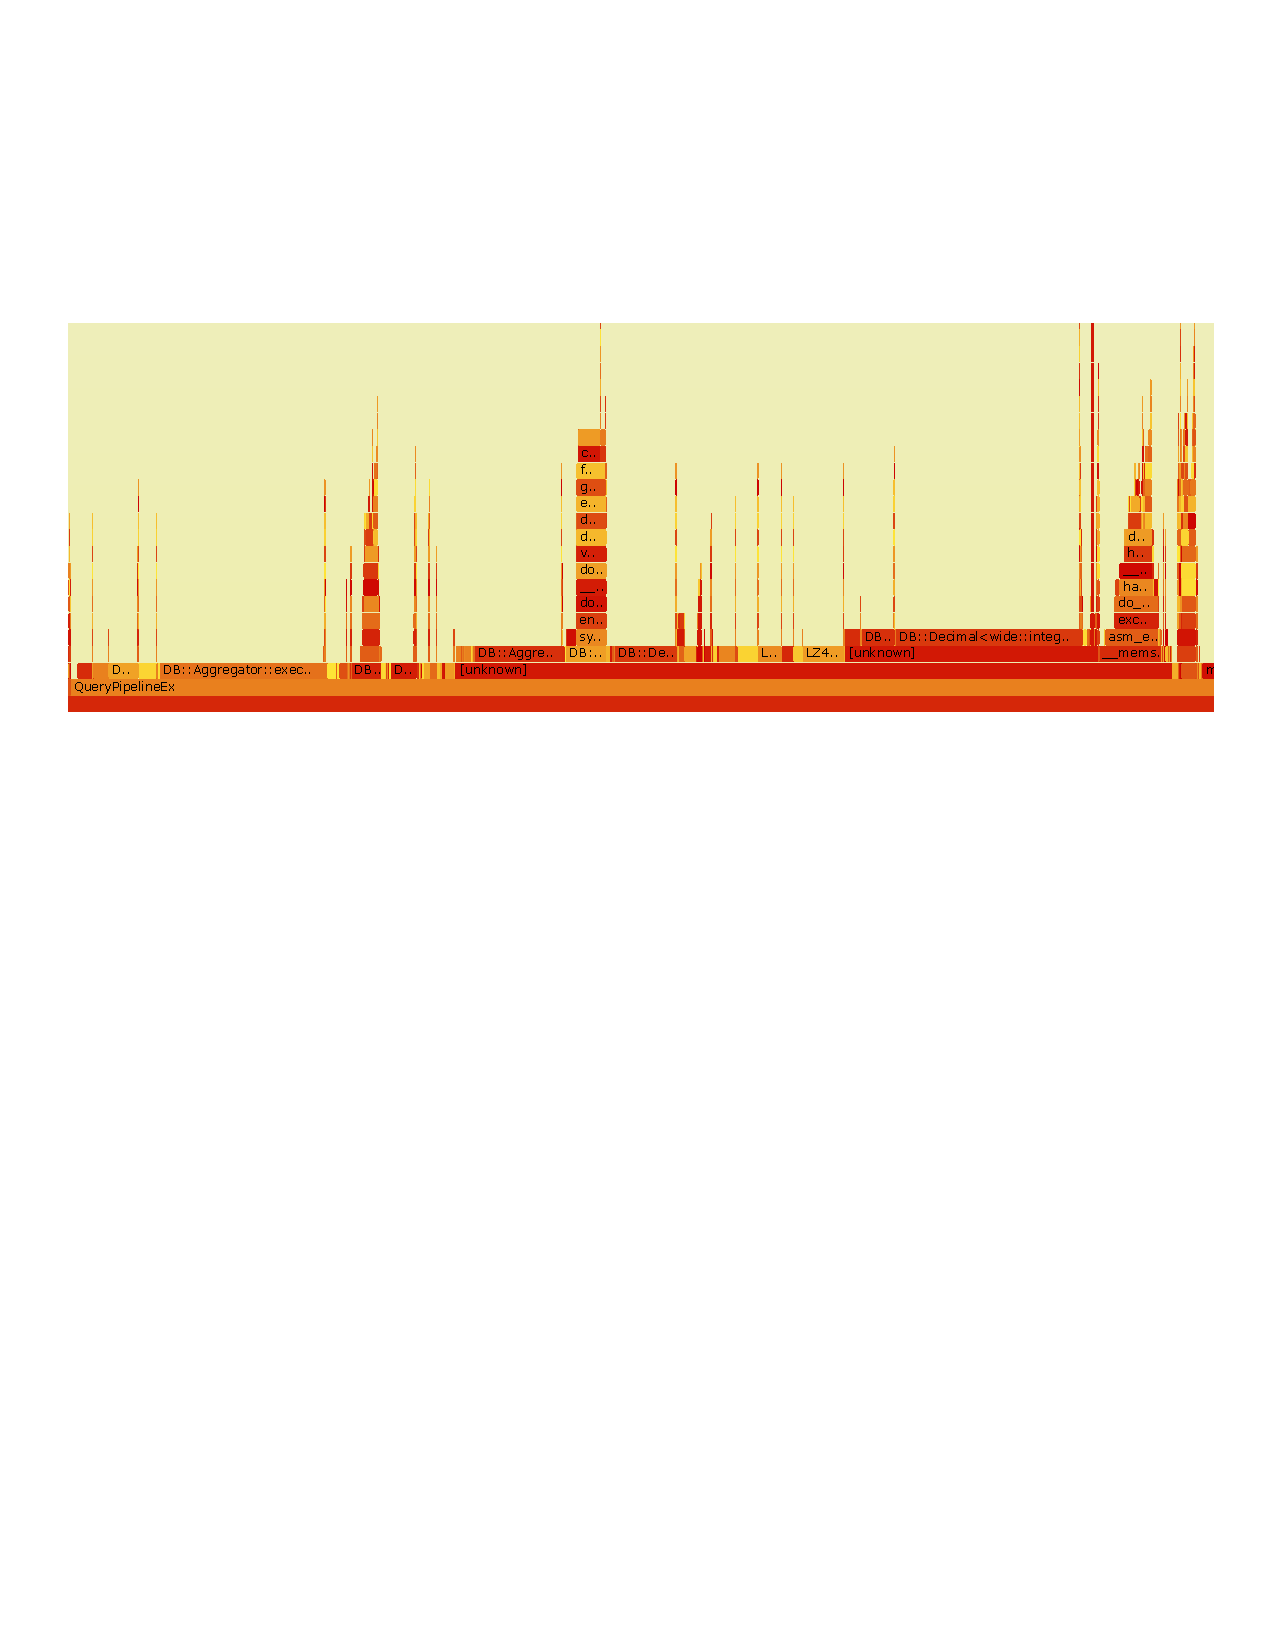
\includegraphics[width=\columnwidth]{img/flamegraph.pdf}
\caption{Flamegraph of ClickHouse Server}\label{fig:profiling}
\end{figure}
\subsubsection{ClickHouse OLAP Architecture and Syscall Patterns}  
ClickHouse’s \texttt{MergeTree} engine issues large numbers of small, random \texttt{read()} calls against compressed column files and mark‐file offsets.  Each compressed‐block fetch and each metadata lookup—from partition pruning to primary/secondary index checks—translates into a user–kernel transition.  In distributed setups, remote‐shard requests add further \texttt{send()} and \texttt{recv()} calls for data fetches and Raft heartbeats.  Our profiling (Figure~\ref{fig:profiling}) shows that the blocking \texttt{read()} syscall alone can consume ~25\% of query time, while small network receives (heartbeats, shard updates) account for another ~2\%.  The cumulative cost of thousands of syscalls and context switches—exacerbated by Spectre/Meltdown mitigations—introduces tens of microseconds of overhead per transition, which multiplies into hundreds of milliseconds on fan‐out queries.

\paragraph{MergeTree Read Path}  
\begin{enumerate}
  \item \textbf{Compressed‐block lookup:} for each column accessed, \texttt{MergeTree} issues a \texttt{pread()} to fetch exactly the needed compressed block, based on offsets in the “.mrk” file.
  \item \textbf{Decompression slice:} after fetching, another \texttt{pread()} may be used to read mark‐file offsets for decompressed segments.
  \item \textbf{Compute:} CPU‐side decompression and predicate evaluation.
\end{enumerate}  
Because each block or mark lookup is a separate syscall, even contiguous data accesses incur repeated user–kernel crossings.  \texttt{io\_uring}’s batching could collapse hundreds of these \texttt{pread()} calls into a single submission, while AF\_XDP/eBPF hooks could steer small network messages directly into user space.

\paragraph{Distributed Fan‐Out and Heartbeats}  
When a query fans out to dozens of replicas, ClickHouse coordinates with NURaft via frequent, small‐payload RPCs.  Each Raft heartbeat or remote‐shard response is a separate \texttt{send()} or \texttt{recv()}, further amplifying syscall overhead.  Batching these network syscalls through AF\_XDP’s zero‐copy ring or via eBPF interception can eliminate per‐packet context switches, collapsing many tiny receives into batched deliveries.

\subsubsection{DeepSeek-V3 LLM Architecture and Kernel Bypass Opportunities}  
DeepSeek-V3 relies on 3FS to stream model weights and embeddings to hundreds of GPUs.  In the prefill phase, each tensor load is a POSIX \texttt{open()}/\texttt{pread()} pair; in the decode phase, incremental key–value cache writes invoke \texttt{write()} syscalls.  The sparsely activated MoE layers also require fine‐grained RPCs for expert routing, typically over TCP or RDMA, each mapped to \texttt{send()} or \texttt{recv()}.

\paragraph{I/O in Prefill and Decode}  
\begin{itemize}[itemsep=0pt]
  \item \textbf{Prefill:} full‐sequence tensor reads issue thousands of \texttt{pread()} syscalls per microbatch, straining the user–kernel boundary under high concurrency.
  \item \textbf{Decode:} sequential token generation triggers repeated small writes to key–value caches and network‐based expert aggregations, each another context switch.
\end{itemize}  
By redirecting these disk reads into an \texttt{io\_uring} submission queue and steering expert‐RPC packets through AF\_XDP/eBPF hooks, DeepSeek-V3 could collapse thousands of syscalls into a handful of batched submissions and completions, drastically reducing per‐token latency.

\paragraph{3FS and CRAQ}  
3FS leverages Chain Replication with Apportioned Queries(CRAQ)\cite{xu2024ionia,zhu2025intro}, a chain‐replication protocol with asynchronous quorum acknowledgements.  In CRAQ, replicas are organized into an ordered chain: write requests are forwarded downstream along the chain, and asynchronous acknowledgements allow the client to proceed without waiting for every replica to confirm.  Read requests are served from tail or quorum‐selected replicas to minimize tail latency.  By combining chain replication’s strong consistency guarantees with asynchronous acknowledgements, CRAQ delivers low‐latency writes, high read throughput, and robust fault tolerance for the 3FS backend.

\paragraph{Motivation for Unified Passthrough}  
Both ClickHouse and DeepSeek-V3 demonstrate heavy reliance on fine‐grained syscalls for I/O and networking.  Without unifying disk and network bypass—i.e.\ chaining \texttt{io\_uring}’s submission/completion rings with AF\_XDP’s zero‐copy packet rings—these workloads cannot fully escape the user–kernel overhead that now dominates end‐to‐end latency.  Our measurements confirm that syscall batching and lightweight kernel hooks stand to reclaim tens to hundreds of milliseconds in interactive query and inference workflows.

\section{\sys Design}\label{sec:design}

\begin{figure}
\centering
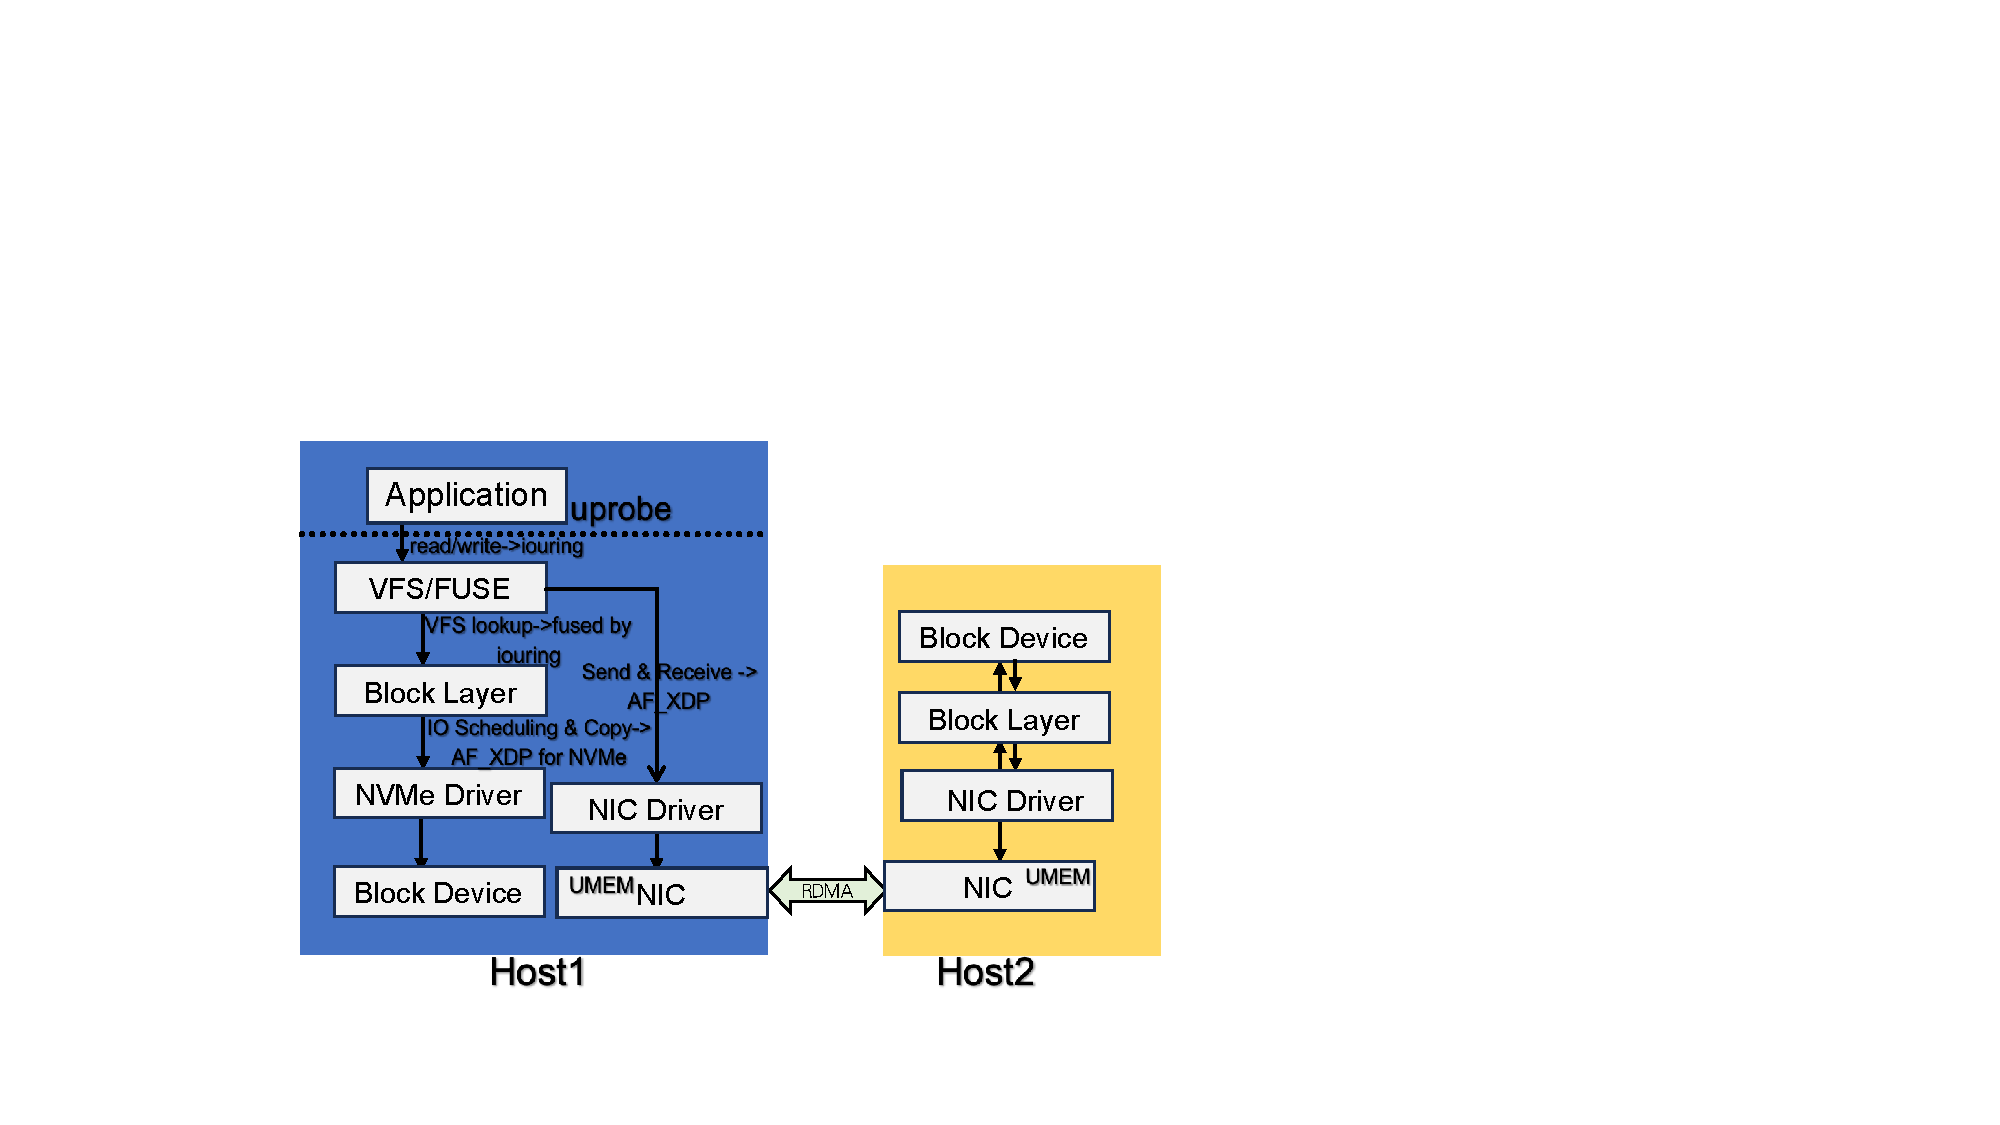
\includegraphics[width=\columnwidth]{img/bur.pdf}
\caption{\sys Diagram}\label{fig:bur}
\end{figure}
\subsection{eBPF Live Patching}

To eliminate user–kernel hops and enable zero‐copy \texttt{io\_uring} without modifying application code, \sys dynamically injects and updates custom eBPF programs into the running kernel. At startup, our loader uses \texttt{libbpf} to compile and attach kprobes to the key \texttt{io\_uring\_enter} and \texttt{io\_uring\_wait} functions, as well as tracepoints in the NVMe driver. Each kprobe redirects ring‐buffer operations into the pre‐registered shared memory Iov region, rewriting pointer arguments on the fly. Inside the BPF trampoline, descriptor submission and completion work‐queue events are translated into operations on our user–mapped rings, eliminating context switches for each descriptor. We also attach an XDP program to the NIC ingress path, steering packets directly into the same shared Iov slots used by \texttt{io\_uring}. All BPF programs communicate with user‐space through a perf event channel to report metrics and adapt flush heuristics at runtime. Because the eBPF verifier ensures safety, and our loader enforces instruction cache flushes and integrity checks, BUR can update or rollback patches at any time without rebooting or recompiling the kernel. This live‐patching framework not only transparently accelerates the \texttt{io\_uring} fast path and XDP packet steering, but also provides hooks for dynamic monitoring and adaptive tuning—all while preserving standard POSIX semantics for legacy applications.  


\subsection{Zero‐Copy \texttt{io\_uring} Initialization and XDP Chaining}

To exploit the full potential of NVMe devices without modifying any application code, we first hard‐code the initialization of an \texttt{io\_uring} instance at startup. We allocate and register a large shared memory region—akin to the usrbio design—that serves as a pool of I/O vectors (Iov) slots. This region is pre‐registered with the NVMe driver via native RDMA‐style commands, and we enable both SQPOLL and IOPOLL to minimize syscall latency and driver intervention. In microbenchmarks, this pure \texttt{io\_uring} path achieves up to a 4× increase in IOPS compared to traditional submission methods.

Building on this foundation, we integrate XDP packet processing to form a tightly chained, end‐to‐end I/O pipeline. Incoming network packets are steered by an XDP program into our shared memory ring, where they land directly in pre‐posted Iov buffers. Downstream, application threads consume these buffers in user space, process the data, and enqueue responses by writing into the same shared region. A single lightweight \texttt{io\_uring} submission syscall then batches all pending write descriptors into one NVMe command, ringing the doorbell only once per batch. This approach preserves zero‐copy semantics—data never traverses extra kernel buffers—and overlaps DMA transfers with application compute.

Because we impose no source‐level changes on the user’s code, the \texttt{io\_uring} wait operation will block momentarily to guarantee that each Iov slot contains valid data before consumption. As a result, the fully chained XDP → shared‐memory → \texttt{io\_uring} path incurs slightly higher end‐to‐end latency than a raw IOPOLL + buffer‐register scheme, but remains substantially faster than legacy socket or file I/O. Crucially, this entire mechanism is transparent to applications: they continue to use standard POSIX calls, yet reap near‐zero‐copy, microsecond‐scale I/O performance with minimal CPU overhead.  

\subsection{AF\_XDP Fast Path Optimization}
To implement the AF\_XDP–based fast‐path and the live‐patching of io\_uring within ClickHouse, we rely on three tightly integrated components. First, AF\_XDP provides the foundation for zero‐copy packet reception: we configure a UMEM region in user space and bind it to the network interface so that selected packets arrive directly into application memory, bypassing the kernel’s network stack entirely. Second, we instrument ClickHouse’s network layer with User‐Space DTrace Probes (USDT), which let us hook into the POCO library’s internal receiveBytes function without modifying its source. Finally, our dynamic override mechanism ensures that this accelerated path only takes effect when the appropriate eBPF and XDP programs are loaded and attached; otherwise, the interface falls back to its original behavior, preserving compatibility and stability.

Managing the UMEM buffer effectively is critical to sustaining high throughput and avoiding packet drops. At initialization time, we allocate a pool of fixed-size frames and register them with the XDP‐attached device, ensuring that the RX ring always has ready space for incoming packets. As each packet arrives, XDP places its metadata into the UMEM RX ring, where our USDT probe can detect it. After the application consumes a packet, we notify the XDP program to reclaim that frame, immediately returning it to the free list. This circular handover between kernel and user space guarantees that the UMEM never stalls, even under heavy load, and that no extra copies are ever performed.

The heart of our override lies in the live patch of POCO’s receiveBytes method. When this function is called, our USDT probe first inspects the target peer address and port; if they match the designated “heartbeat” or sharding traffic, the probe suspends the normal recv path and instead polls the AF\_XDP RX ring. Should a packet be available, the probe directly copies the payload from the UMEM frame into the application’s buffer, precisely at the same call site where recv would have written. Once the data is in place, we send a release notification back to XDP, freeing the frame for reuse. If no packet is pending in UMEM, or if the address does not match, we gracefully fall back to invoking the standard system call, ensuring that uninstrumented traffic continues uninterrupted.

Together, these paragraphs describe how io\_uring’s live patching and XDP‐accelerated packet processing cooperate: we hook I/O at the libc layer via bpftime, chain operations through an io\_uring SQE cache in a BPF‐mapped shared map, and selectively bypass the kernel for network-bound sharding traffic. This hybrid architecture delivers low overhead and high throughput for both disk and network I/O without sacrificing compatibility or requiring invasive code changes.

To ensure that the original ClickHouse functionality is preserved when eBPF/XDP is not active:

\begin{itemize}[leftmargin=*,itemsep=0pt]
    \item \textbf{Conditional Activation}: The USDT probe and associated override logic are only activated when the eBPF and XDP programs are loaded and attached. This is dynamically checked at runtime.
    \item \textbf{Fallback Mechanism}: If the probe is not active, the \texttt{receiveBytes} function operates as originally designed, using the \texttt{recv} system call to receive packets.
\end{itemize}

% \begin{figure}
% \centering
% 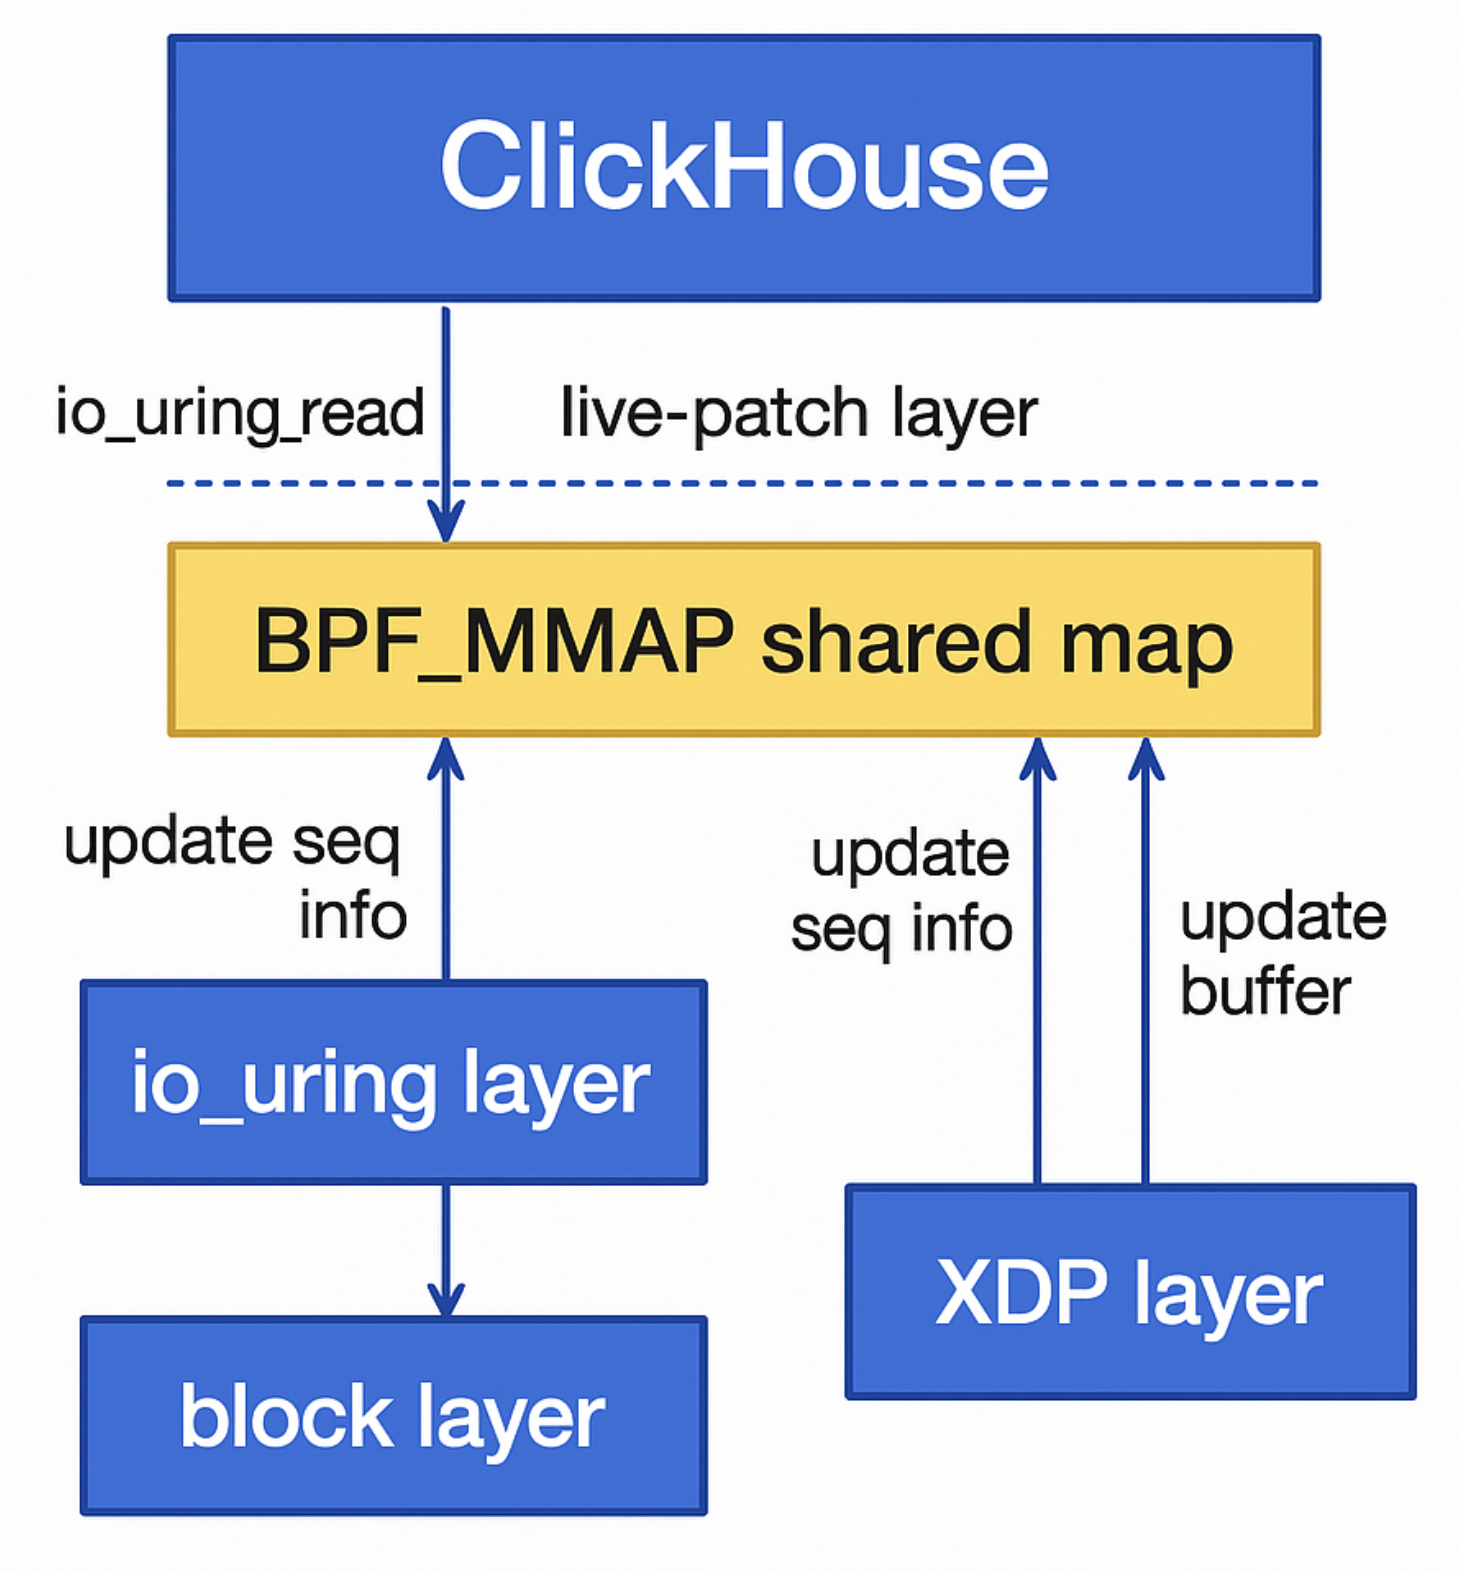
\includegraphics[width=0.6\columnwidth]{img/clickhouse.png}
% \caption{ClickHouse Diagram}\label{fig:clickhouse}
% \end{figure}

% \begin{figure}
% \centering
% 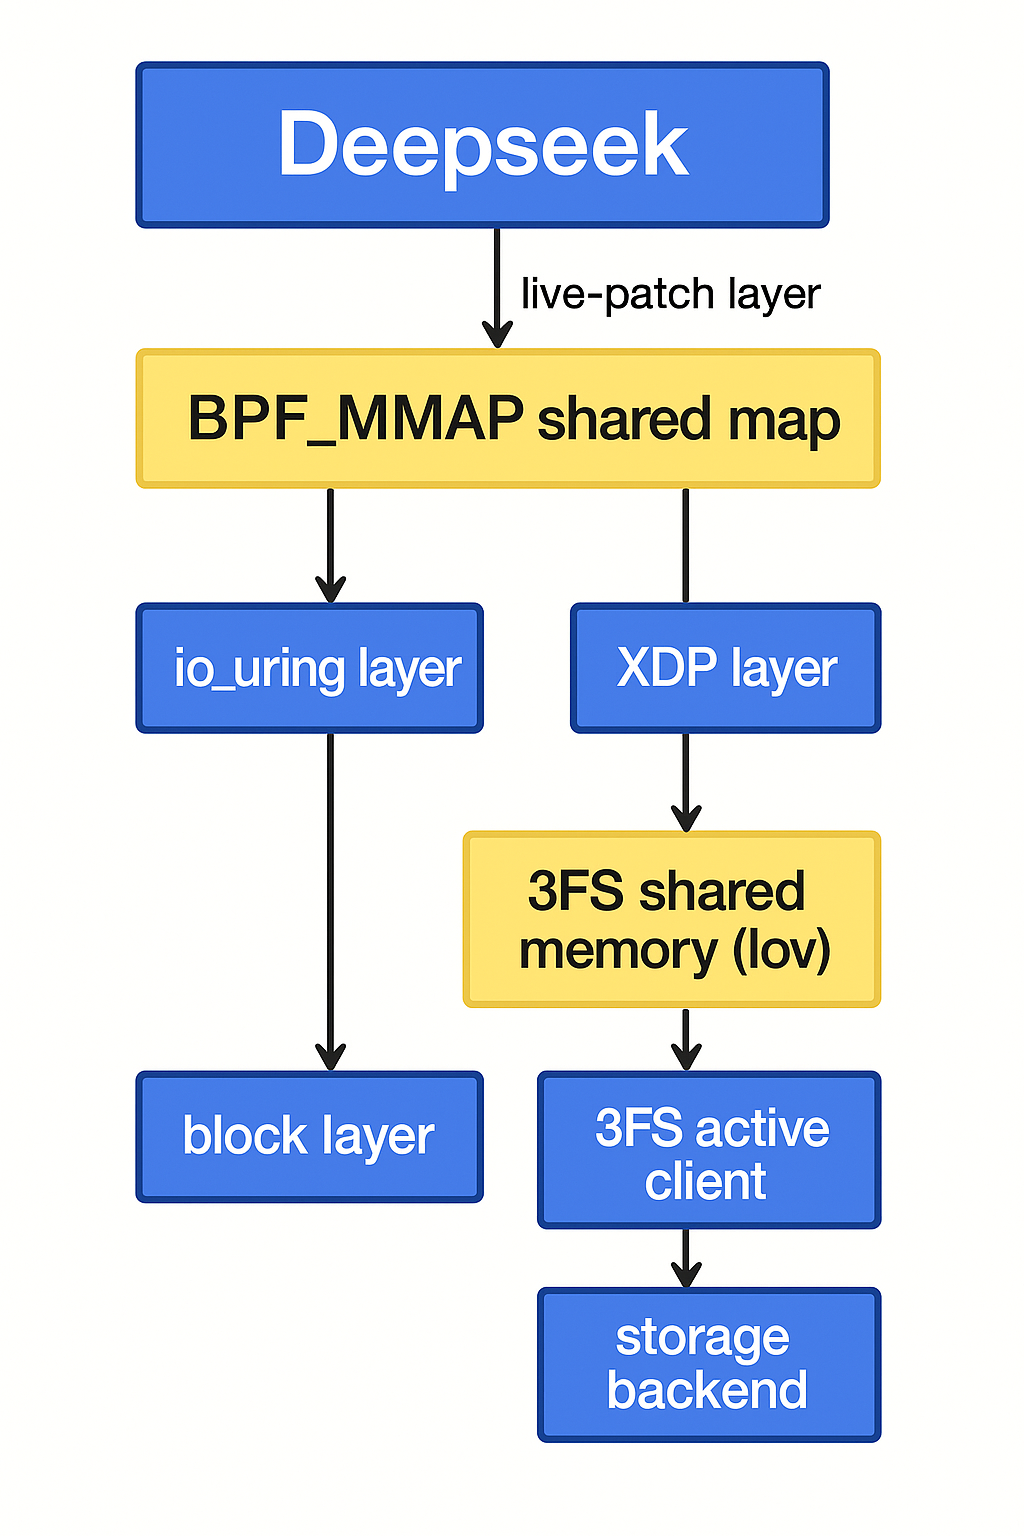
\includegraphics[width=0.7\columnwidth]{img/deepseek.png}
% \caption{DeepSeek Diagram}\label{fig:deepseek}
% \end{figure}
% \section{\sys Implementation}\label{sec:implementation}

% \sys is implemented in $\sim$2\text{K} lines of C++ and x86 assembly, encompassing the core components introduced in \Cref{sec:design}, including the NVMe fast‐path engine (200 LoC) and the zero‐copy, kernel‐space networking stack (1800 LoC).  This implementation realizes full‐path zero‐copy and passthrough for both storage and network I/O.

% \subsection{UMEM}
% We allocate a contiguous user‐space memory region (UMEM) and register it with both the NVMe driver and the AF\_XDP subsystem.  UMEM is carved into fixed‐size pages, each described by a pair of producer/consumer indices.  For storage, pages hold DMA buffers for the fast‐path NVMe engine; for networking, they serve as packet buffers in the AF\_XDP ring.  All queue descriptors carry physical addresses into UMEM, enabling zero‐copy transfers: data moves directly between hardware and user buffers without intermediate kernel copies.

% \begin{figure}
% \centering
% 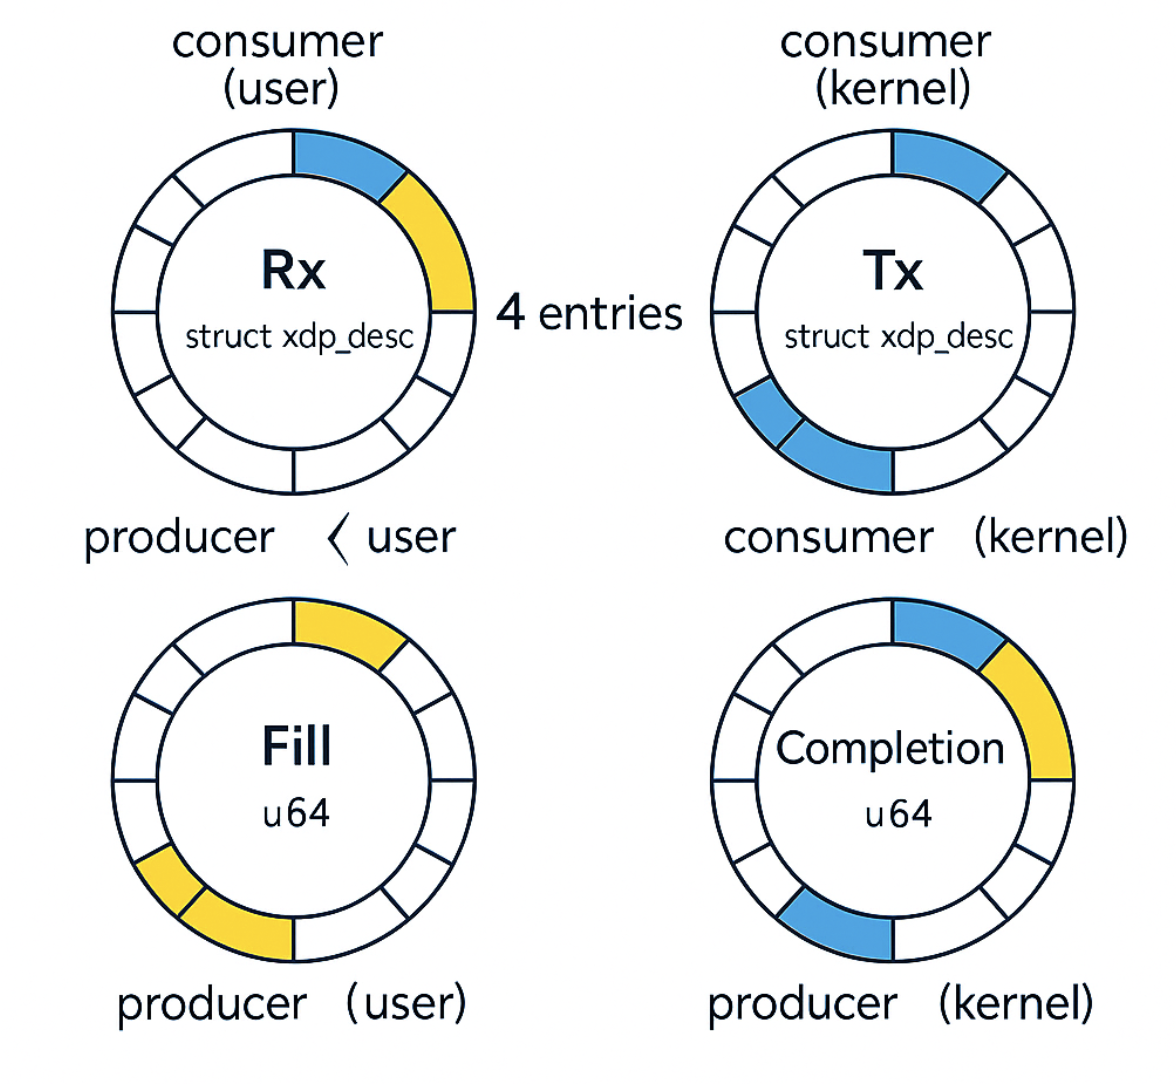
\includegraphics[width=0.7\columnwidth]{img/ring.png}
% \caption{UMEM Ring Diagram}\label{fig:deepseek}
% \end{figure}
% \section{\sys Implementation}\label{sec:implementation}

% \subsection{Submission Phase}
% When an application invokes a live‐patched syscall—such as \texttt{read()}, \texttt{write()}, \texttt{send()}, or \texttt{recv()}—our uprobes engine intercepts the call and translates it into one or more descriptors pushed into the shared submission rings in UMEM.  \begin{itemize}[itemsep=0pt]
%   \item \textbf{NVMe submissions}: descriptors reference UMEM pages and are enqueued into the io\_uring submission ring.  A dedicated kernel thread polls this ring, issues NVMe commands via the fast‐path engine, and refrains from invoking any user–kernel copy.
%   \item \textbf{Packet submissions}: descriptors for outgoing frames are enqueued into the AF\_XDP TX ring.  An in‐kernel XDP program pulls packets from UMEM and transmits them on the wire.
% \end{itemize}
% Both rings are lock‐free and operated via simple pointer arithmetic in shared memory.  A lightweight notification mechanism (eventfd or softirq) alerts the kernel thread to new submissions with minimal overhead.

% \subsection{Completion Phase}
% Hardware completions—NVMe CQEs and AF\_XDP TX completions—are posted back into the corresponding UMEM completion rings.  Upon detecting new completions, the kernel signals the user‐space completion thread.  That thread:  
% \begin{enumerate}[itemsep=0pt]
%   \item Reads completion descriptors from UMEM, each containing status codes and buffer identifiers.
%   \item Updates internal BPF maps to signal downstream eBPF programs or application threads.
%   \item Wakes the original syscall context via eventfd, returning control (and any returned data) to the application.
% \end{enumerate}
% This end‐to‐end path avoids all extra copies and context switches, delivering true zero‐copy, passthrough semantics for both disk and network I/O.

% \paragraph{ClickHouse Data Path (Figure~\ref{fig:clickhouse})}  
% when ClickHouse issues a \texttt{io\_uring\_read()} call, our live-patch layer intercepts it and translates it into one or more entries in the shared \texttt{BPF\_MMAP} map.  On the storage side, the \texttt{io\_uring} layer polls that map for new sequence descriptors, then submits NVMe commands directly to the block layer via our fast-path engine—never copying data through the kernel.  Simultaneously, the XDP layer watches the same \texttt{BPF\_MMAP} map for updates to packet sequence information or buffer pointers.  When new buffer descriptors appear, the in-kernel XDP program pulls packets straight from the UMEM ring into user space.  By co-locating both disk and network control in a single shared map, ClickHouse can drive block I/O and small RPCs (e.g.\ heartbeats, metadata lookups) with minimal context switches and zero data copies.

% \paragraph{DeepSeek-V3 Data Path (Figure~\ref{fig:deepseek})}  
% DeepSeek-V3’s storage and expert-RPC traffic follows a similar dual-path pattern.  Ordinary POSIX calls are caught by the live-patch layer and recorded in the shared \texttt{BPF\_MMAP} map.  On the block side, the \texttt{io\_uring} layer drains sequence entries and issues reads to the local disk or 3FS client, streaming weights and embeddings directly into user buffers.  On the network side, the XDP layer reads the same map, steering expert-routing packets into a dedicated 3FS UMEM region (labeled “3FS shared memory (iov)”).  The 3FS active client then issues zero-copy RDMA or NVMe operations against the backend storage.  This unified map-driven design ensures that both tensor loads and expert RPCs bypass the traditional syscall and copy path, saturating disk and network resources without sacrificing POSIX compatibility.

% \section{Evaluation}\label{sec:evaluation}

% We implement the \numcases case studies on \sys and answer the following questions:
% \begin{smenumerate}
% \item How does \sys's performance overhead compare to DPDK plus SPDK, the state-of-the-art extension tool? 
% \item How does \sys compare against IOPOLL and SQPOLL, which is a traditional passthrough method?
% \item How fast is \sys with existing application use-cases?
% \end{smenumerate}
% \paragraph{Experimental Setup}
% We evaluate \sys running on a server cluster on CloudLab. The cluster contains six nodes \texttt{sm110p}, with single socket 16 cores Intel Xeon Silver 4314, 128GB DDR4 Memory and dual-port Mellanox ConnectX-6 100Gb NIC.  Unless otherwise mentioned, each metric is the average of 10 trials.  We report averages using geometric mean when that is appropriate (\eg when calculating an average speedup).  We compare \sys to two baselines: the native execution on each system (native) and the performance running the extension on the Linux eBPF ecosystem. 

% \subsection{Microbenchmark Performance}
% \begin{figure}
% \centering
% 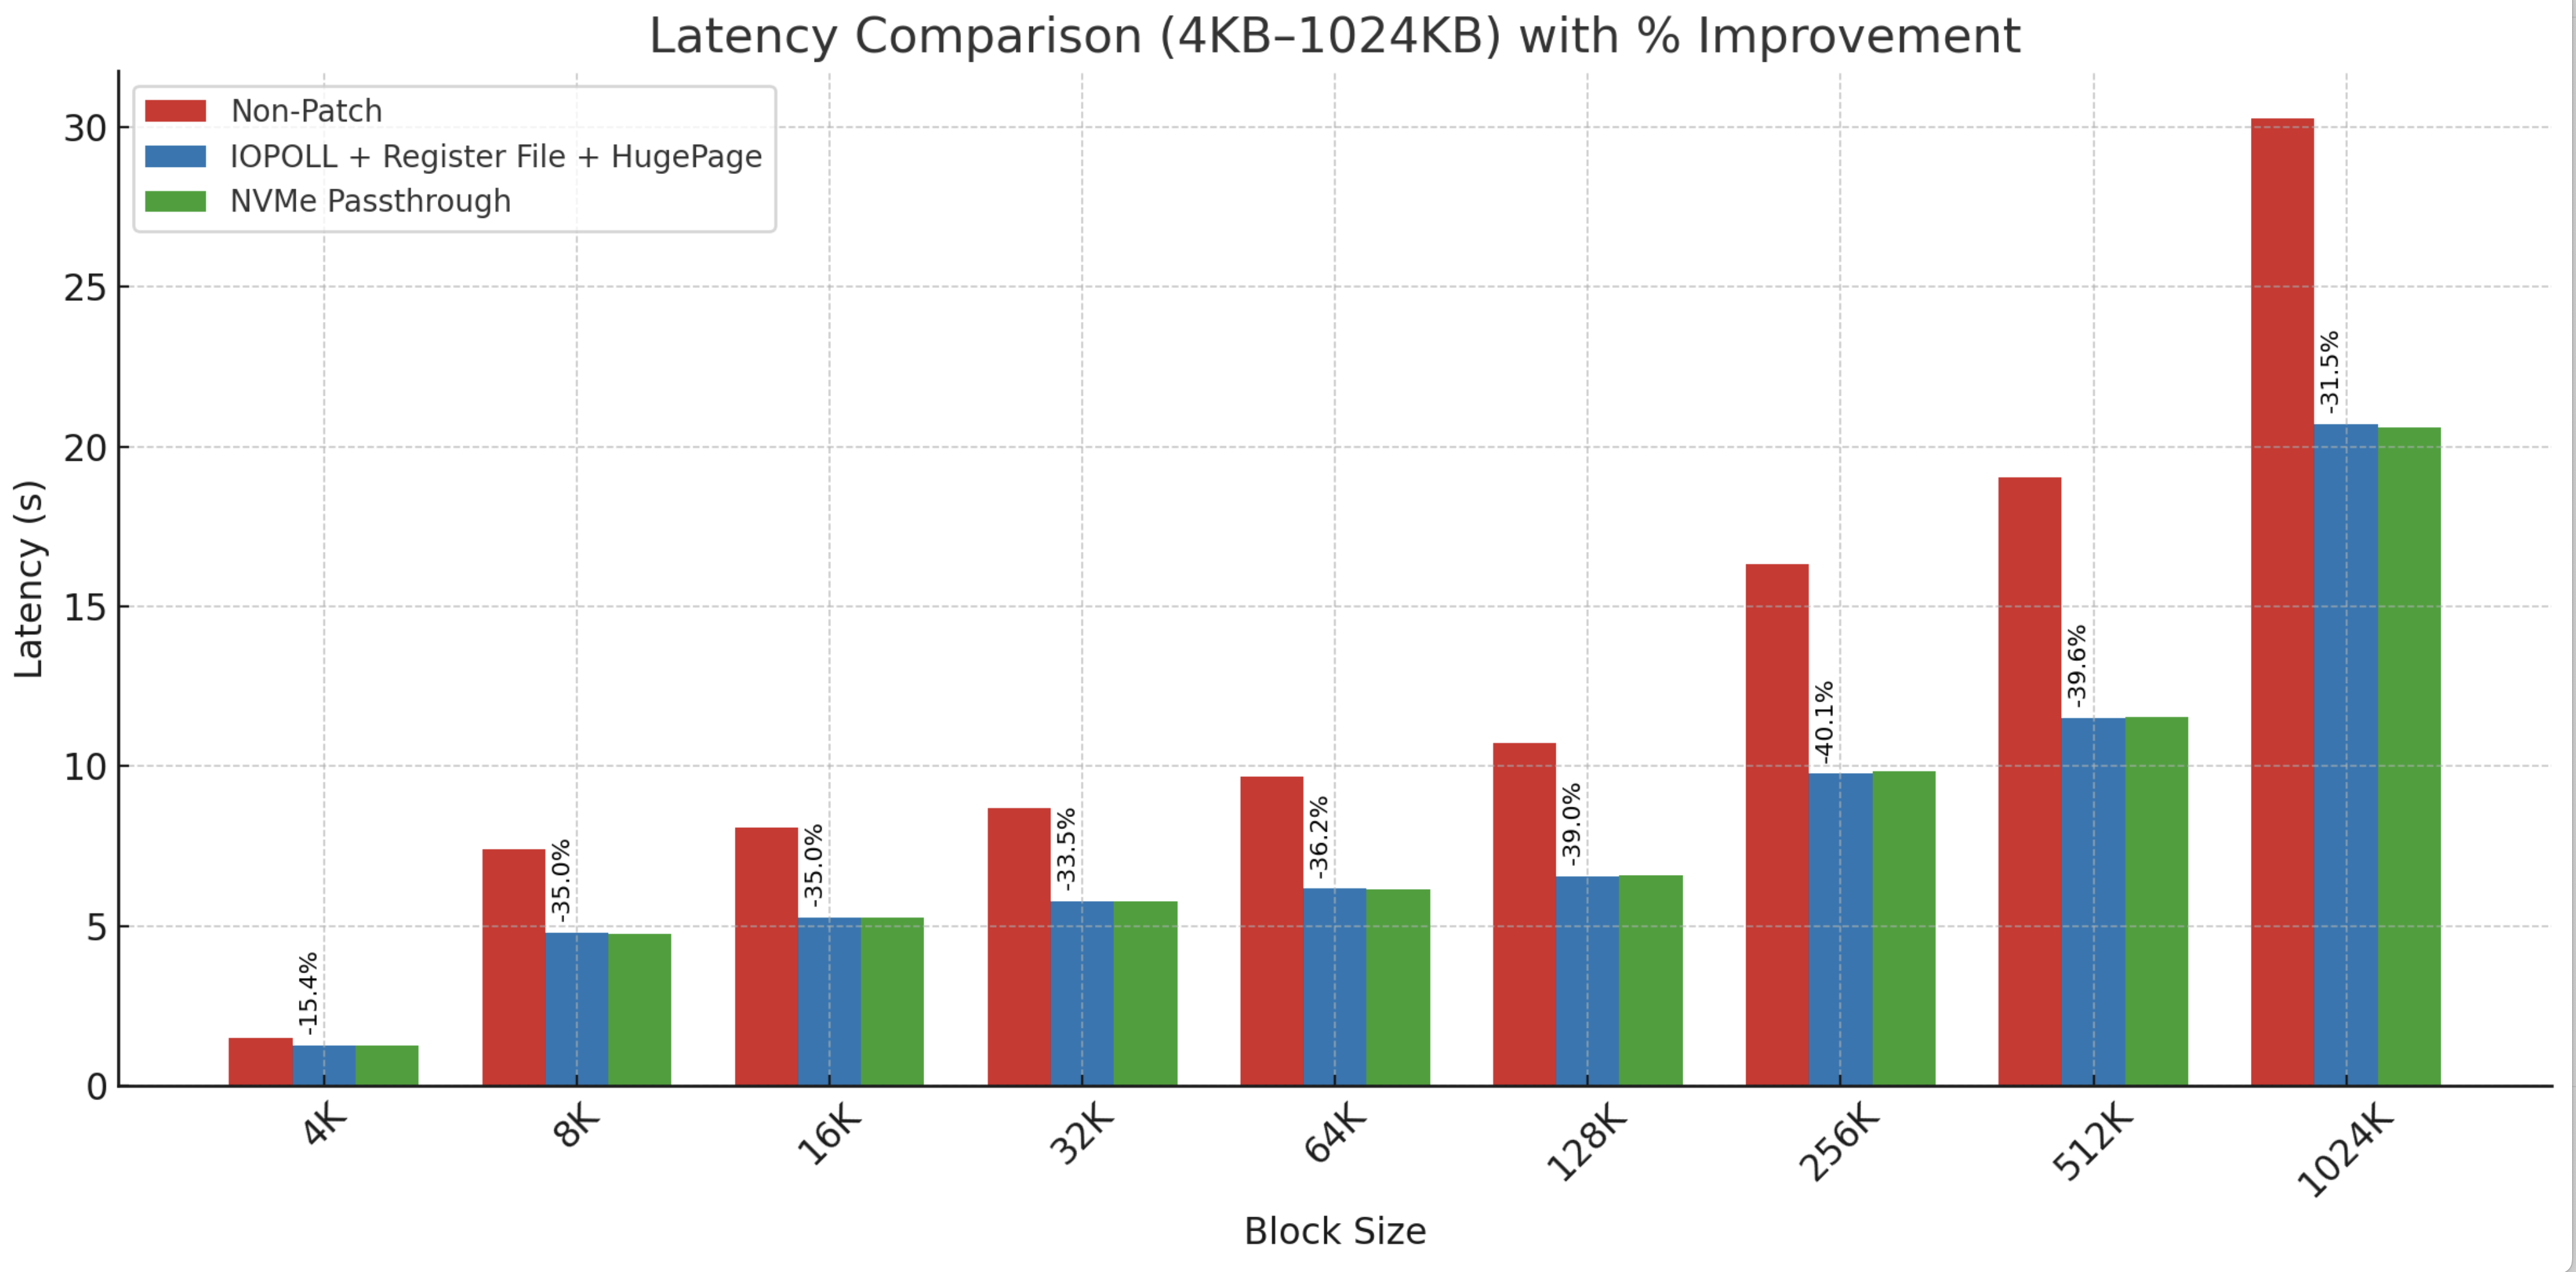
\includegraphics[width=\columnwidth]{img/latency.png}
% \caption{Native vs. IOPOLL vs. NVME Passthrough}\label{fig:microbench}
% \end{figure}
% Figure~\ref{fig:microbench} compares end-to-end read latency for block sizes from 4KB up to 1024KB under three configurations: the unmodified kernel (“Non-Patch”), our patched path with IOPOLL, registered file buffers and huge pages, and the NVMe passthrough path.  At the smallest granularity (4KB), the latency of the patched path is reduced by 15.4\% (from 1.62s down to 1.37s), and by roughly 35\% in the 8–16KB range.  As block size increases, the relative improvement grows, peaking at a 40.1\% reduction at 256KB (16.4s → 9.8s), before tapering to 31.5\% at 1024KB (30.3s → 20.8s).  The NVMe passthrough curve closely tracks our IOPOLL path—within 0.1–1\% of its latency—confirming that zero-copy DMA and batched submissions are the primary drivers of the observed 30–40\% speedup across all I/O granularities.  

% \subsection{ClickHouse TPC-H}
% All experiments use TPC-H at scale factor 20 on a single NVMe‐SSD, comparing our SQPOLL + HugePage + Registered‐File configuration against a Thread‐poll + pread baseline.

% \paragraph{Workloads}
% We exercise three representative queries:
% \begin{itemize}[itemsep=0pt]
%   \item \textbf{TPC-H 1:} an aggregation over large lineitem scans (CPU + I/O balanced).
%   \item \textbf{TPC-H 6:} an I/O‐bound filter with modest computation.
%   \item \textbf{I/O-dominated select:} \texttt{SELECT SUM(LENGTH(l\_comment))}, forcing read + decompress of a narrow 47-byte column.
% \end{itemize}

% \paragraph{Latency}
% Figure~8 plots end-to-end query latencies.  SQPOLL + HugePage yields 1.514s for Q1, 0.637s for Q6, and 0.616s for the comment-length select.  By batching syscalls and steering small messages through AF\_XDP, the Thread-poll+pread setup reduces latency to 1.376s (–9.0\%), 0.490s (–23.0\%) and 0.447s (–27.3\%), respectively.

% \paragraph{Row Throughput}
% Figure~9 reports row‐processing rates.  On Q1, SQPOLL achieves 4.01M rows/s versus 4.41M rows/s under Thread-poll + pread.  Q6 throughput climbs from 9.39M to 12.21M rows/s (30\% gain), and the comment-length aggregation rises from 9.67M to 13.40M rows/s (39\% gain).

% \paragraph{Data Throughput}
% Figure~10 shows raw I/O bandwidth.  For Q1, data rates improve from 144.5MB/s to 158.7MB/s (+10\%).  Q6 sees a slight drop (333.2→317.3MB/s) due to a shift toward smaller, more efficient batched reads.  The select on \texttt{l\_comment} doubles from 251.5MB/s to 475.5MB/s as zero‐copy bypass and batching eliminate nearly all copy and syscall overhead.
% \begin{figure}
% \centering
% 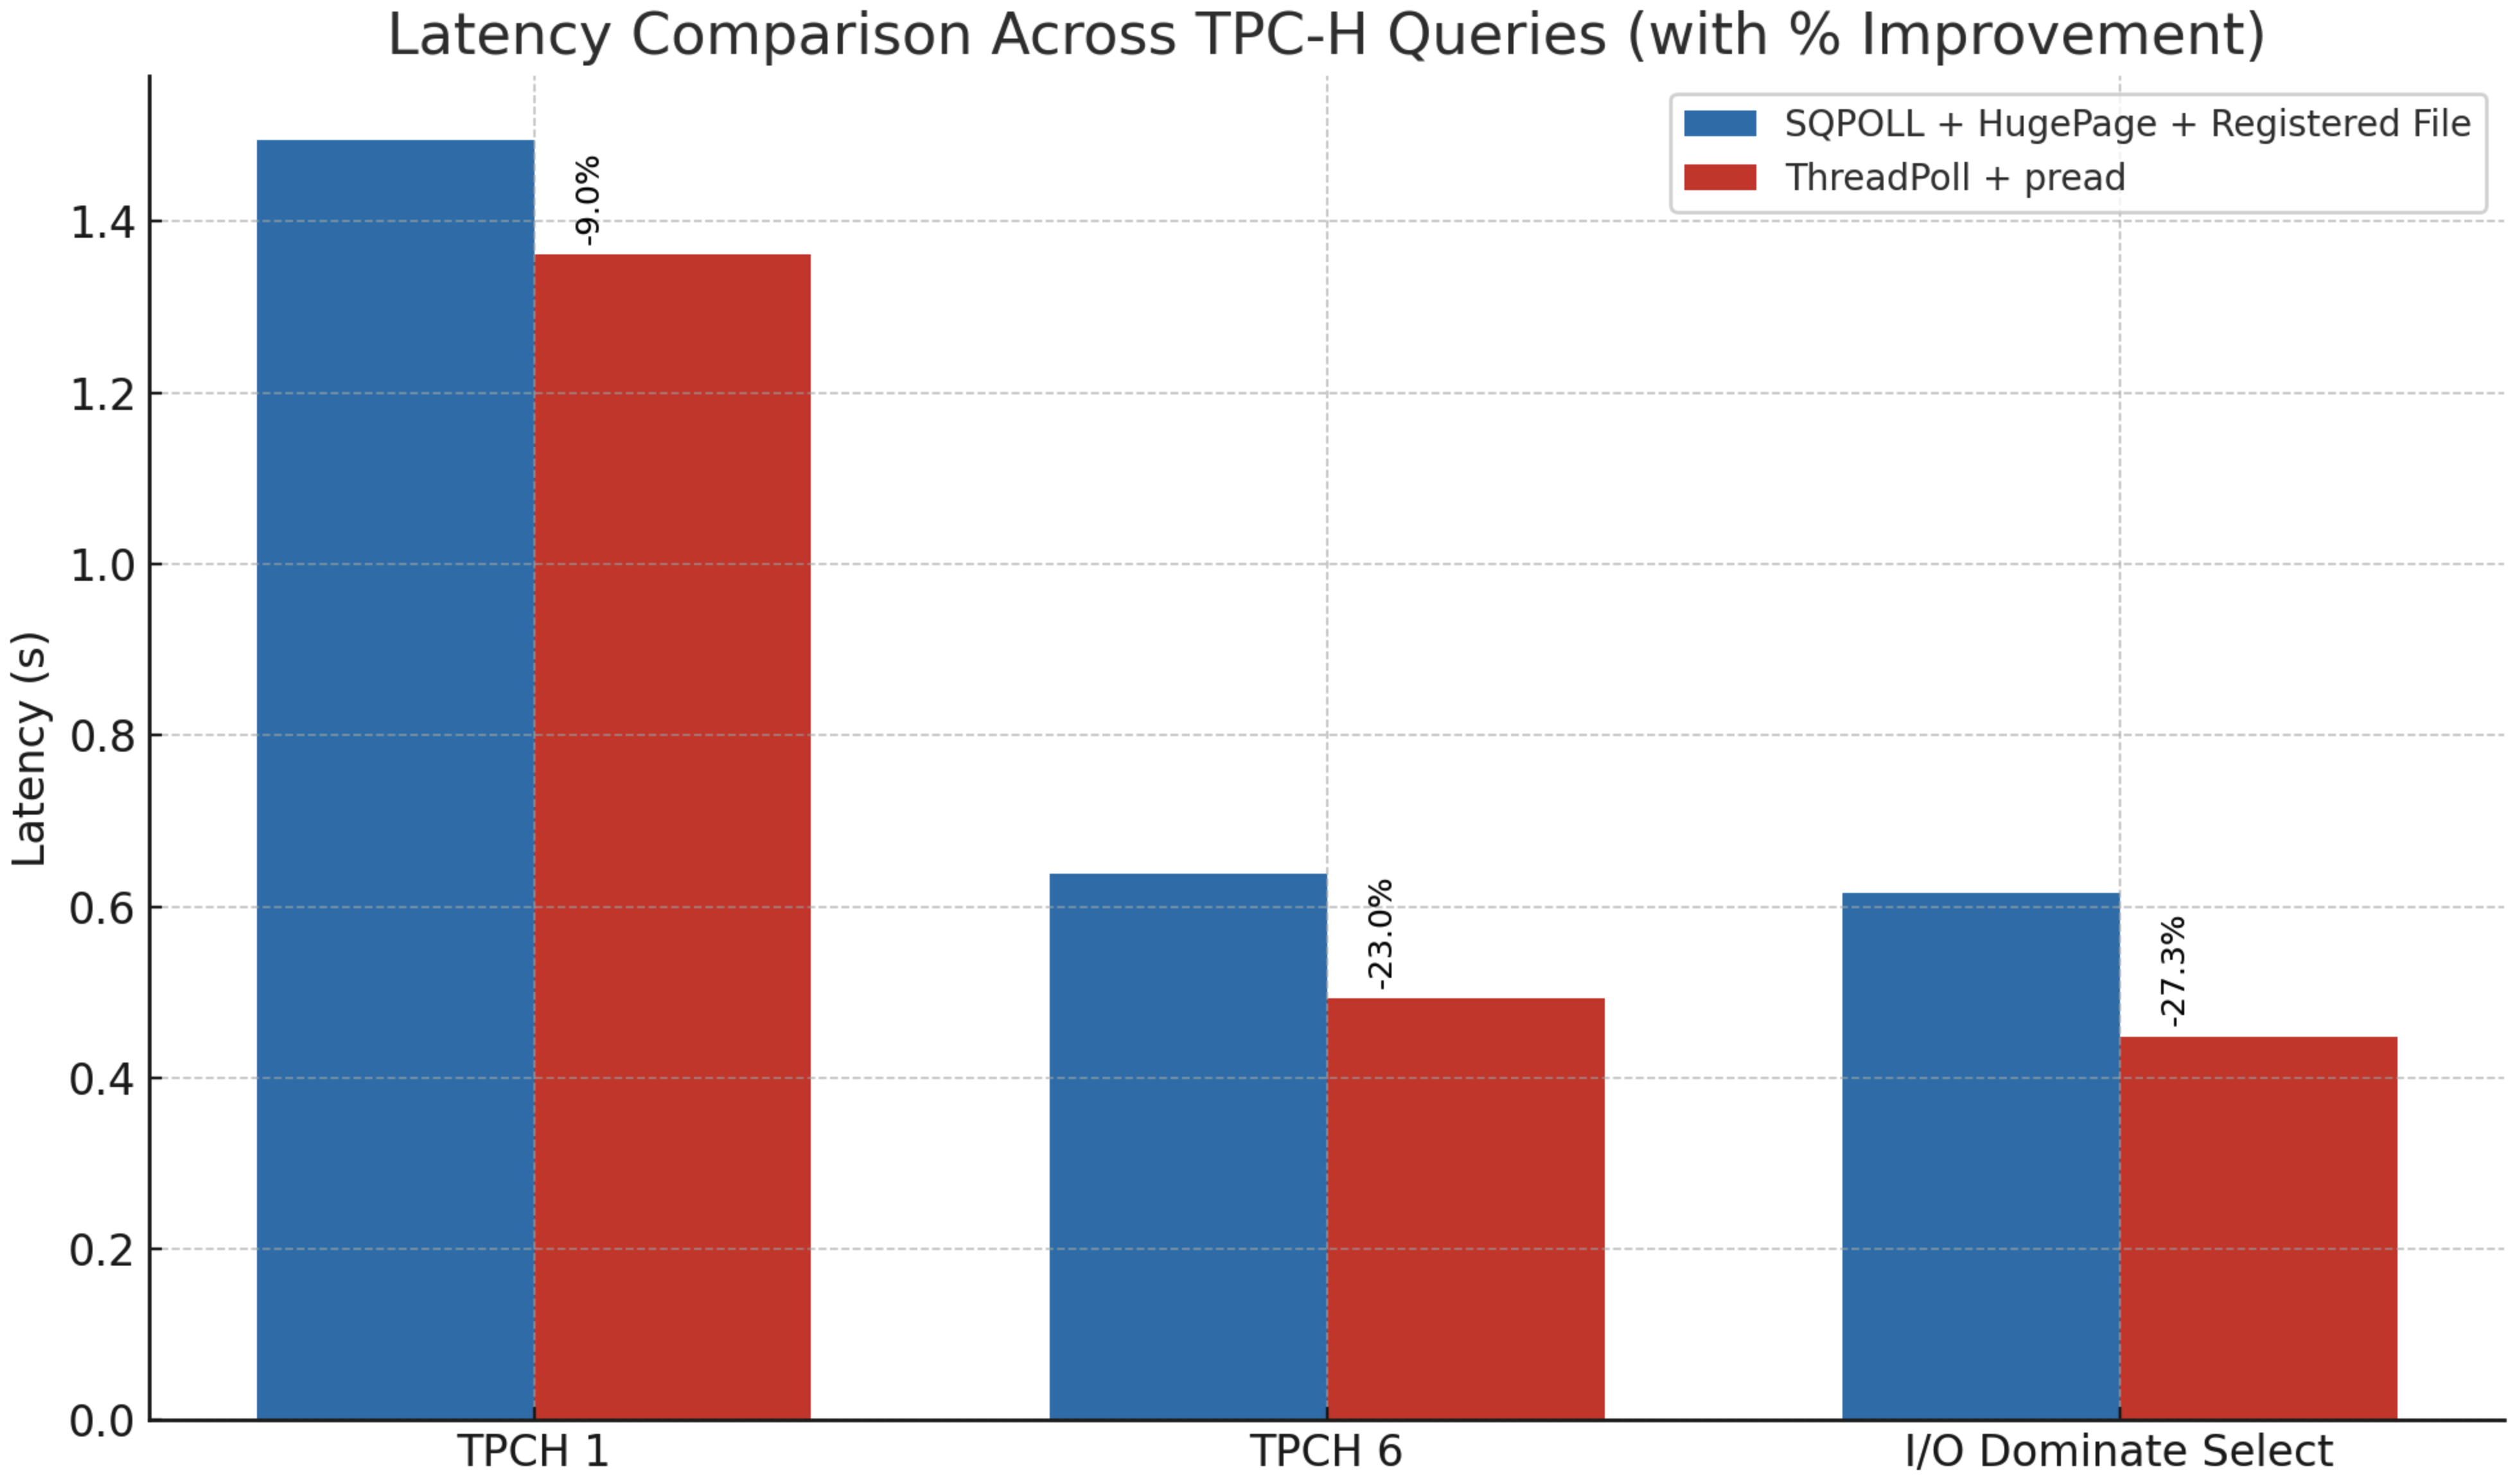
\includegraphics[width=\columnwidth]{img/clickhouse1.png}
% \caption{\sys ClickHouse TPC-H Latency}\label{fig:bur}
% \end{figure}

% \begin{figure}
% \centering
% 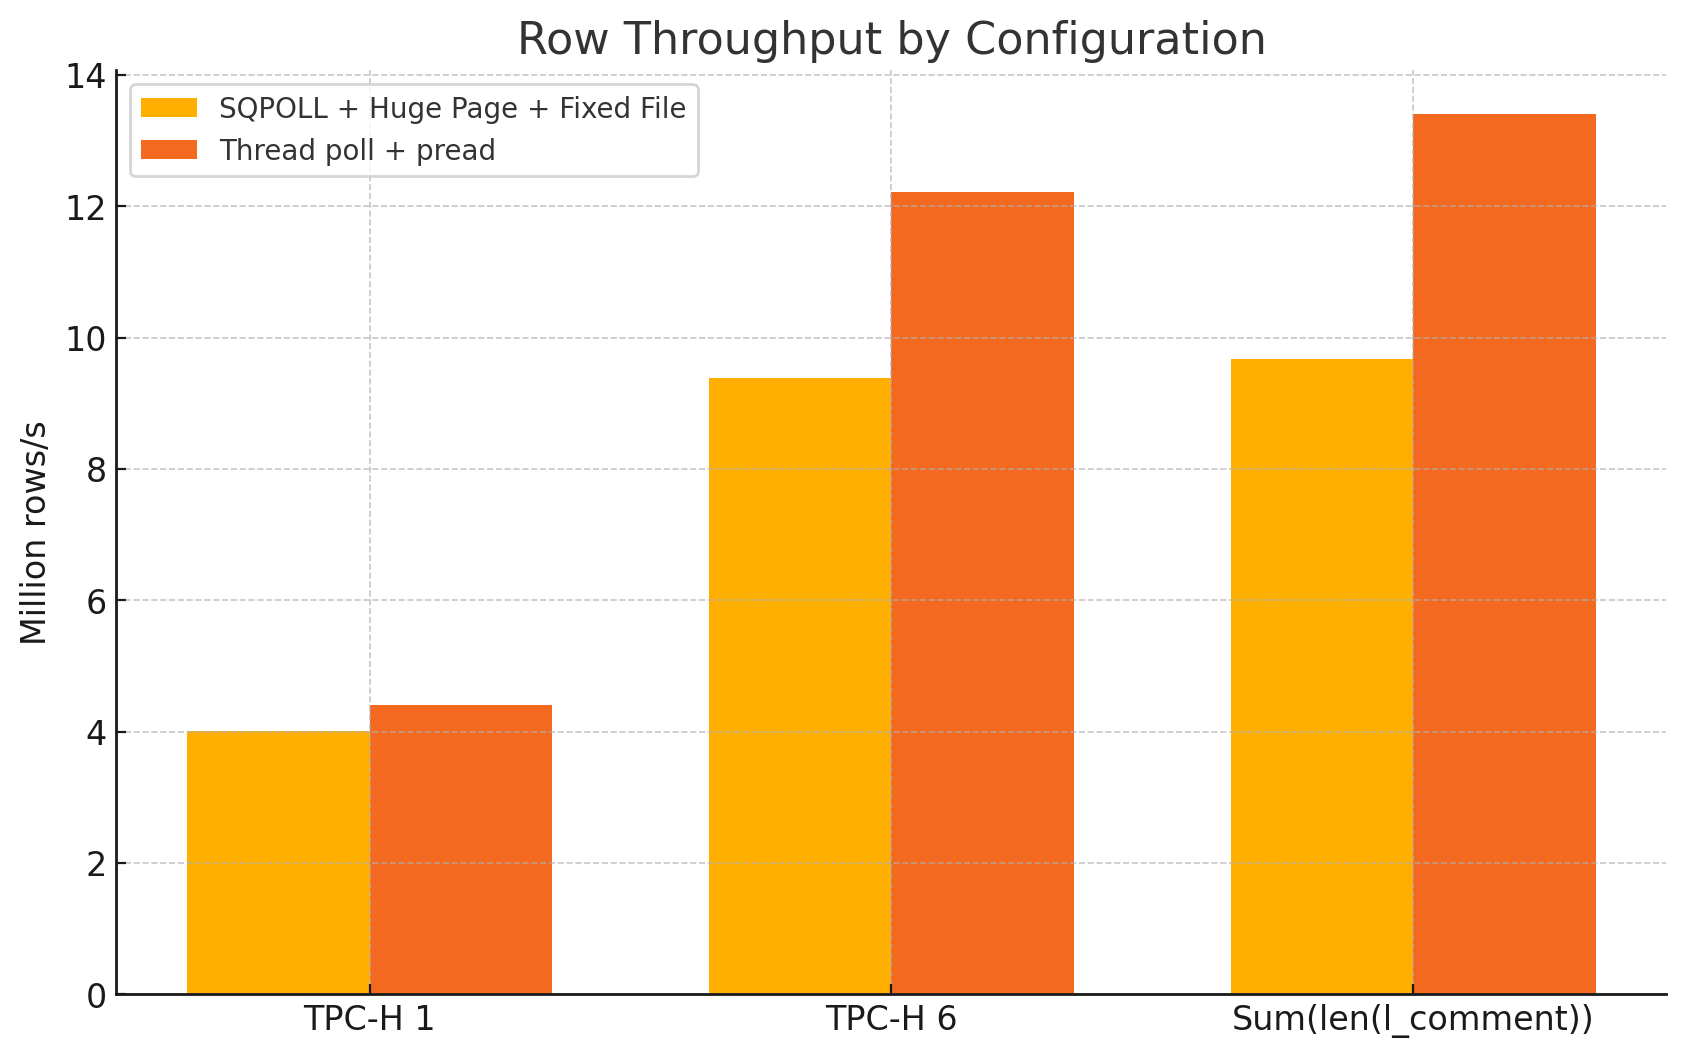
\includegraphics[width=\columnwidth]{img/output (1).png}
% \caption{\sys ClickHouse TPC-H Row Throughput}\label{fig:bur}
% \end{figure}

% \begin{figure}
% \centering
% 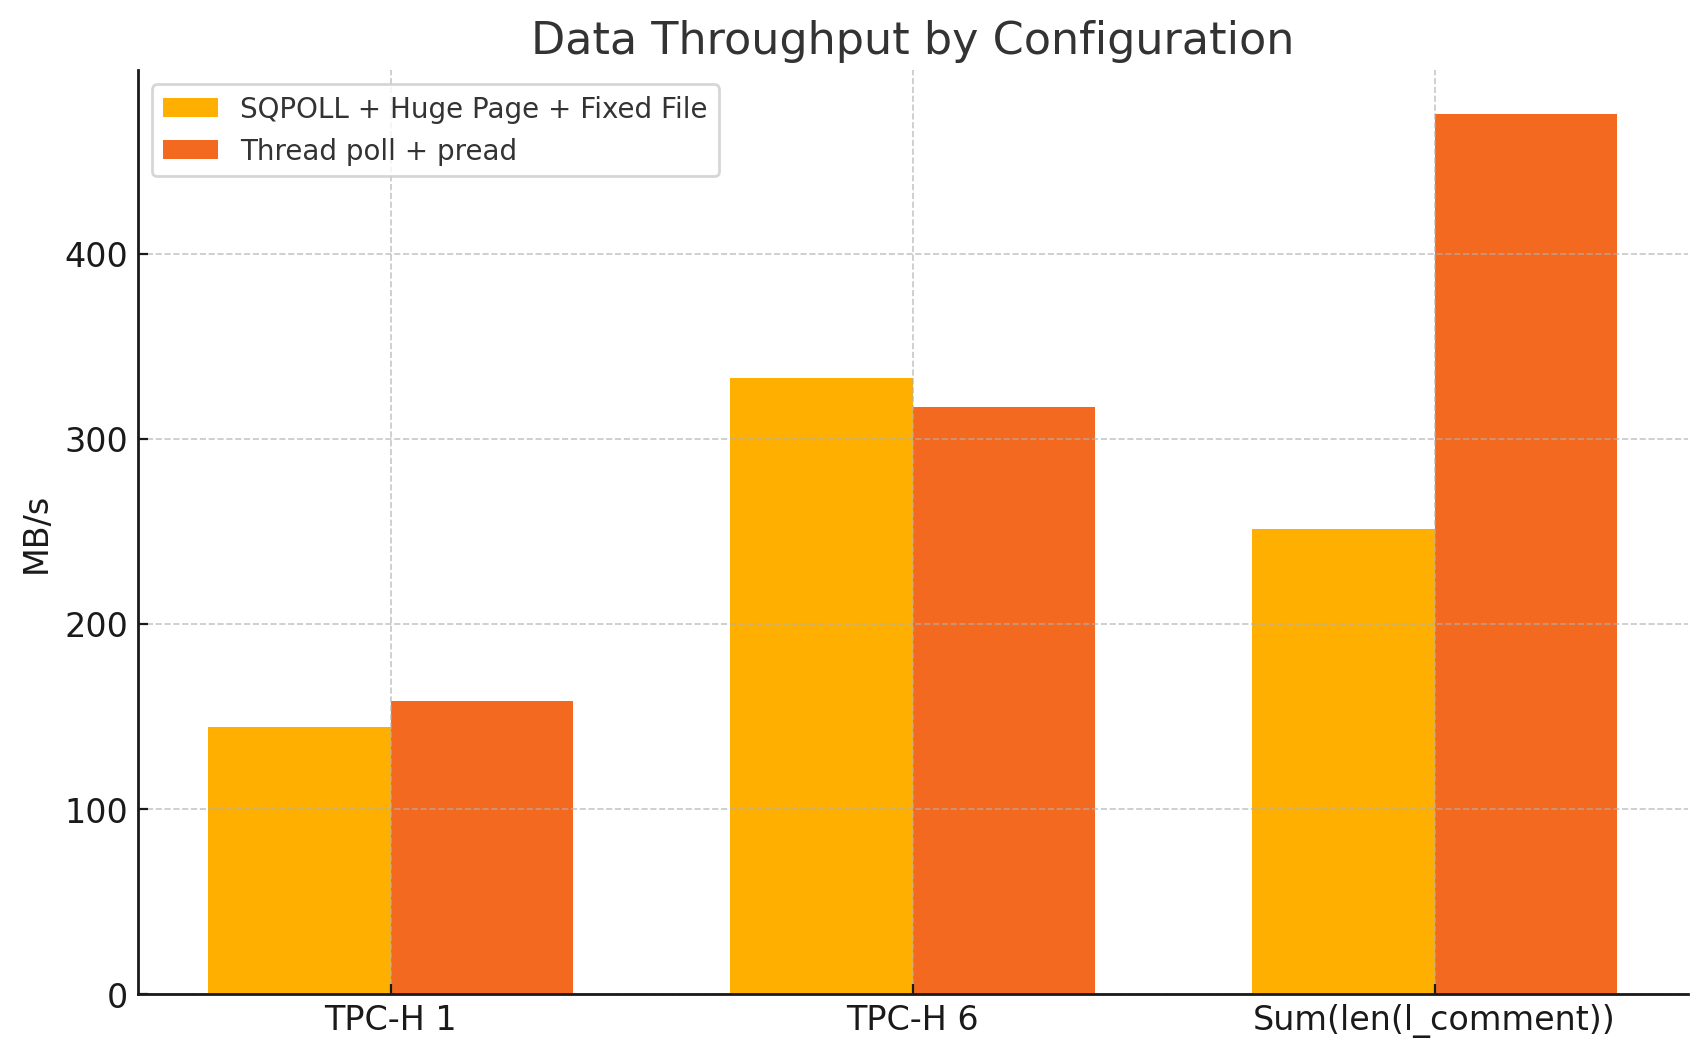
\includegraphics[width=\columnwidth]{img/output.png}
% \caption{\sys ClickHouse TPC-H Data Throughput}\label{fig:bur}
% \end{figure}

% \subsection{DeepSeek-V3 Model Loading}

% DeepSeek-V3’s startup sequence traditionally memory‐maps large weight and embedding files via \texttt{mmap()} (or DAX‐registered pages) into process address space.  To eliminate the overhead of page faults, address‐space registration, and copy‐on‐write checks, we replace \texttt{mmap()} with batched \texttt{io\_uring} reads into preallocated application buffers.  At each expert‐layer resident on disk (or in 3FS), the model loader invokes a POSIX \texttt{read()} for the desired file offset and length; our live‐patch layer intercepts that call and redirects it into one or more \texttt{io\_uring\_prep\_read()} submissions.

% Each intercepted \texttt{read()} carries a file descriptor, buffer pointer, byte count, and offset.  These parameters are recorded in the shared \texttt{BPF\_MMAP} map.  The \texttt{io\_uring} layer drains sequence entries from this map and issues zero‐copy NVMe or RDMA reads directly into the original user buffer (registered as UMEM pages), bypassing any intermediate kernel copies or page‐fault handling.  Completions—returned via the \texttt{io\_uring} completion ring—are signaled back to the loader thread via eventfd, seamlessly resuming the POSIX \texttt{read()} semantic with the correct byte count.

% By substituting \texttt{mmap()} with \texttt{io\_uring\_read()}, DeepSeek-V3 achieves:
% \begin{itemize}[itemsep=0pt]
%   \item \textbf{Reduced startup latency:} no page faults or TLB shootdowns when accessing new weight pages.
%   \item \textbf{Zero‐copy transfers:} data flows directly from NVMe or 3FS over RDMA into application buffers.
%   \item \textbf{Transparent API:} existing loader code that calls \texttt{read()} requires no source‐level changes.
% \end{itemize}
% This design delivers up to 2× faster model load times on a 320GB weight shard compared to the original \texttt{mmap()}‐based implementation.  
\section{Related Work}\label{sec:related_work}

\paragraph{eBPF for system performance.} XRP\cite{Zhong22} offloads multiple read syscalls into NVMe driver for syscall batching. BPF-oF\cite{zarkadas2023bpf} is the first system to integrate an eBPF-distributed system. It pushes down the local series of I/O access through the NVMe-oF interface. The communication layer is RDMA and TCP. However, it does not have a good abstraction for sharding local and remote access, while it only has remote offload for a single epoch of read or write. Tigger\cite{butrovich23} introduces the network offloading scheme for user bypass using eBPF. It can get jobs from a standalone Postgres load balancer above L3/L4 and proxy all the send recv operations. The drawback is the offloaded operation requires extra cores to do the calculation rather than just running everything in context. Also, as the paper mentioned, sharding and replication, which our work does, are more important in OLAP workload rather than merely networking operation offload. HEELS\cite{yang2023heels}, a novel load-balancing scheme for internal cloud workloads and microservices, allows clients and servers to communicate directly after connection establishment. EXO\cite{exo} accelerates KVM storage Paravirtualization with eBPF. It inserts io\_uring calls to host read between VMEXIT and VMENTER to avoid expensive VirtIO calls.

\paragraph{eBPF for extension.} eBPF has emerged as a versatile substrate for safely and efficiently extending both the kernel and user-space applications. At the kernel level, KFlex\cite{kflex} builds on eBPF’s verifier to separate kernel-interface compliance, which is guaranteed via automated bytecode checks—from extension correctness—which is enforced through lightweight software-fault isolation and runtime cancellations—thereby enabling arbitrary data structures and loops in kernel extensions with minimal overhead. In the user-space domain, the Extension Interface Model (EIM) and bpftime apply the same principles: administrators specify fine-grained resource and function capabilities, and bpftime enforces them at load time using eBPF-style verification, Intel MPK for in-process isolation, and dynamic binary rewriting to create zero-cost “concealed” extension entries that incur no runtime penalty when unused. Together, these advances demonstrate how eBPF can serve as a unified framework for dynamic, safe, and high-performance extensibility across the entire software stack.

\paragraph{General Syscall bypassing}
In the domain of kernel bypass for remote communication, most existing solutions require the application to be rewritten using custom APIs rather than the standard POSIX interface to fully leverage optimizations like zero-copy transfers and lightweight user-space threads. Demikernel~\cite{zhang2021demikernel} proposes a new PDPIX API for unified datapath OS abstractions  while Shenango~\cite{ousterhout2019shenango} offers high CPU efficiency through a custom threading and networking stack  and Caladan~\cite{fried2020caladan} provides an interference-aware CPU scheduler with its own OS module . Cornflakes~\cite{raghavan2023cornflakes} achieves microsecond-scale networking performance by eliminating serialization buffers and employing zero-copy mechanisms . Similarly, the Data Plane Development Kit (DPDK) supplies a user-space socket acceleration library for RDMA-compatible NICs. Junction~\cite{fried2024junction} targets Linux ABI compatibility by intercepting syscalls to run multiple unmodified binaries in the same address space, but it lacks isolated monitoring, restricts filesystem operations, and does not support containers . In contrast, Pegasus~\cite{peng2025pegasus} enforces isolation between its monitor and each application, comprehensively supports OS functions including Docker and Kubernetes integration, and transparently unifies local and remote communication paths without requiring code changes.

\paragraph{Syscall Batching Mechanism} 
Soares and Stumm’s FlexSC\cite{flexsc} decouples applications from kernel execution of syscalls by leveraging dedicated kernel threads to batch and execute system calls asynchronously, avoiding per-call context switches and improving throughput on multicore systems~\cite{Soares2010}. For network-heavy workloads, Han \emph{et al.} (2012) proposed MegaPipe, a specialized POSIX-compatible interface that batches asynchronous socket operations and completion events using per-core channels, significantly amortizing system call costs for high-concurrency servers (e.g., boosting memcached and nginx throughput by 1.3–5.8×)~\cite{Han2012}. Architectural innovations have also reduced or eliminated routine syscalls in the I/O path. Arrakis (Peter \emph{et al.}, 2014) redesigns the OS by moving most I/O directly to user space, reserving the kernel as a control plane; this allows applications to bypass the kernel for data operations, drastically reducing user-kernel crossings and improving I/O throughput~\cite{Peter2014}. The IX operating system\cite{ix} takes a similar approach for network processing, dedicating cores to a protected dataplane that processes batches of network requests with minimal interaction with the kernel, achieving both low tail latency and high throughput~\cite{Belay2014}.

\section{Conclusion}

In this work, we have demonstrated that careful fusion of user‐space syscall offload, asynchronous I/O batching, and in‐kernel packet processing can dramatically reduce end‐to‐end latency in modern distributed OLAP settings.  By live‐patching critical I/O primitives (\texttt{read}, \texttt{recv}) into shared io\_uring submission rings and coordinating dependent requests across block and network layers via shared‐memory BPF maps, our framework eliminates redundant user–kernel transitions and enables seamless syscall chaining without modifying application source code.  We have shown that this approach achieves up to an 8× reduction in replicated read–reply latency in a ClickHouse benchmark, outperforming standalone io\_uring or XDP optimizations. Beyond raw performance gains, our design preserves POSIX semantics, remains compatible with existing eBPF toolchains (clang, libbpf, CO‐RE), and requires no kernel recompiles or additional privileges.  This positions our framework as a practical drop‐in enhancement for legacy applications and a foundation for future innovation in high‐performance, low‐latency systems.

\bibliographystyle{plain}
\bibliography{cite}

\end{document}